\section{第二讲：原子结构}\label{ux7b2cux4e8cux8bb2ux539fux5b50ux7ed3ux6784}

\subsection{学习目标}\label{ux5b66ux4e60ux76eeux6807}

\begin{itemize}
\tightlist
\item
  能说出原子结构模型从 Dalton 到量子力学的关键发展节点及其实验依据
\item
  能复述Bohr模型三假设，推导氢原子光谱公式，计算Balmer系谱线波长
\item
  能用德布罗意关系式 \(\lambda = h/p\) 计算实物粒子的波长，用测不准原理解释''轨道''概念的失效
\item
  能用四个量子数描述原子中电子的运动状态，判断量子数组的合法性
\item
  能写出薛定谔方程的一般形式（直角坐标），理解波函数 \(\psi\) 的概率诠释
\item
  能运用构造原理、Pauli不相容原理和Hund规则写出Z≤54元素及常见离子的基态电子排布
\item
  能解释Cr、Cu等元素电子排布特例（半满/全满稳定化），并能迁移至Mo、Ag、Pd等特例
\item
  能区分离子失电子顺序与原子电子填充顺序的区别，正确写出过渡金属离子的排布
\item
  能运用Slater规则计算指定电子的屏蔽常数 \(\sigma\) 和有效核电荷 \(Z^*\)，估算轨道能量
\item
  能读取Cotton能级图，理解填充顺序与轨道真实能量的区别
\item
  能对照原子半径/电离能/电负性趋势图，解释周期律反常点
\item
  能用 \(Z^*\) 的定量变化解释同周期元素性质的递变规律
\end{itemize}

\subsection{一、原子结构模型的发展}\label{ux4e00ux539fux5b50ux7ed3ux6784ux6a21ux578bux7684ux53d1ux5c55}

\textbf{关联知识点}：原子结构 · 原子轨道

\subsubsection{1.1 从经典到量子：一场跨越两千年的认知跃迁}\label{ux4eceux7ecfux5178ux5230ux91cfux5b50ux4e00ux573aux8de8ux8d8aux4e24ux5343ux5e74ux7684ux8ba4ux77e5ux8dc3ux8fc1}

原子模型的演变史，本质上是一部''人类如何用实验逼出微观真相''的认识论教材。每一代模型都是对上一代局限性的突破------\textbf{不是旧模型错了，而是它只在特定精度下成立}。下表梳理了关键跃迁：

{\def\LTcaptype{none} % do not increment counter
\begin{longtable}[]{@{}
  >{\raggedright\arraybackslash}p{(\linewidth - 8\tabcolsep) * \real{0.2000}}
  >{\raggedright\arraybackslash}p{(\linewidth - 8\tabcolsep) * \real{0.2000}}
  >{\raggedright\arraybackslash}p{(\linewidth - 8\tabcolsep) * \real{0.2000}}
  >{\raggedright\arraybackslash}p{(\linewidth - 8\tabcolsep) * \real{0.2000}}
  >{\raggedright\arraybackslash}p{(\linewidth - 8\tabcolsep) * \real{0.2000}}@{}}
\toprule\noalign{}
\begin{minipage}[b]{\linewidth}\raggedright
模型
\end{minipage} & \begin{minipage}[b]{\linewidth}\raggedright
提出者（年份）
\end{minipage} & \begin{minipage}[b]{\linewidth}\raggedright
核心假设
\end{minipage} & \begin{minipage}[b]{\linewidth}\raggedright
实验依据
\end{minipage} & \begin{minipage}[b]{\linewidth}\raggedright
致命缺陷
\end{minipage} \\
\midrule\noalign{}
\endhead
\bottomrule\noalign{}
\endlastfoot
\textbf{实心球模型} & Dalton（1803） & 原子不可再分 & 倍比定律、定组成定律 & 未揭示内部结构 \\
\textbf{葡萄干布丁模型} & Thomson（1903） & 正电荷均匀分布，电子散在其中 & 阴极射线→发现电子 & 无法解释α散射 \\
\textbf{核式模型} & Rutherford（1911） & 核（正+质量）+ 核外电子 & α粒子散射：1/8000偏转\textgreater90° & 经典电磁→电子坠核 \\
\textbf{玻尔模型} & Bohr（1913） & 定态轨道 + 跃迁辐射 & 氢原子线状光谱（Balmer系） & 无法解释精细结构+多电子 \\
\textbf{量子力学模型} & Schrödinger（1926） & 电子由 \(\psi\) 描述，\(\|\psi\|^2\) 为概率密度 & 德布罗意波粒二象性 + 电子衍射 & --- \\
\end{longtable}
}

📌 \textbf{理解要点}：``如果电子绕核做圆周运动，根据经典电磁理论------加速运动的电荷会辐射电磁波。辐射→能量损失→速度降低→轨道缩小→最终坠入原子核。但原子明明是稳定的------这是经典物理给量子论的第一个耳光。''

\textbf{拓展：核反应与放射性} ------ Rutherford 的alpha散射实验不仅揭示了原子核的存在，也是核反应研究的起点。常见的核反应类型包括：

{\def\LTcaptype{none} % do not increment counter
\begin{longtable}[]{@{}
  >{\raggedright\arraybackslash}p{(\linewidth - 4\tabcolsep) * \real{0.3333}}
  >{\raggedright\arraybackslash}p{(\linewidth - 4\tabcolsep) * \real{0.3333}}
  >{\raggedright\arraybackslash}p{(\linewidth - 4\tabcolsep) * \real{0.3333}}@{}}
\toprule\noalign{}
\begin{minipage}[b]{\linewidth}\raggedright
类型
\end{minipage} & \begin{minipage}[b]{\linewidth}\raggedright
通式
\end{minipage} & \begin{minipage}[b]{\linewidth}\raggedright
示例
\end{minipage} \\
\midrule\noalign{}
\endhead
\bottomrule\noalign{}
\endlastfoot
\(\alpha\) 衰变 & \(\ce{^{A}_{Z}X -> ^{A-4}_{Z-2}Y + ^{4}_{2}He^{2+}}\) & \(\ce{^{238}_{92}U -> ^{234}_{90}Th + ^{4}_{2}He^{2+}}\) \\
\(\beta\) 衰变 & \(\ce{^{A}_{Z}X -> ^{A}_{Z+1}Y + ^{0}_{-1}e^{-}}\) \(+ \bar{\nu}_e\) & \(\ce{^{14}_{6}C -> ^{14}_{7}N + ^{0}_{-1}e^{-}}\) \(+ \bar{\nu}_e\) \\
\(\gamma\) 辐射 & \(\ce{^{A}_{Z}X^{*} -> ^{A}_{Z}X}\) \(+ \gamma\) & \(\ce{^{60}_{27}Co^{*} -> ^{60}_{27}Co}\) \(+ \gamma\) \\
\end{longtable}
}

核反应涉及原子核内部的变化（质子数或中子数的改变），与核外电子排布本质上是不同物理层次的问题。

\textbf{理解方法论}：以上每一种模型都经历了''\textbf{实验异常 → 旧模型失效 → 新假设提出 → 数学形式化 → 新预言被验证}''的循环。这不仅是原子结构的发展史，更是科学思维的标准模板。

\subsubsection{1.2 玻尔模型：旧量子论的巅峰与天花板}\label{ux73bbux5c14ux6a21ux578bux65e7ux91cfux5b50ux8bbaux7684ux5dc5ux5cf0ux4e0eux5929ux82b1ux677f}

\paragraph{① 问题的起点：氢原子光谱为什么是线状的？}\label{ux95eeux9898ux7684ux8d77ux70b9ux6c22ux539fux5b50ux5149ux8c31ux4e3aux4ec0ux4e48ux662fux7ebfux72b6ux7684}

按照经典电磁学，电子绕核做圆周运动会不断辐射电磁波，能量持续损失，轨道半径连续缩小，最终坠入原子核。这意味着原子光谱应该是\textbf{连续谱}------就像白炽灯的光谱一样。然而实际观测到的氢原子光谱却是\textbf{线状的}------只有特定波长的谱线。

\begin{figure}[H]\centering
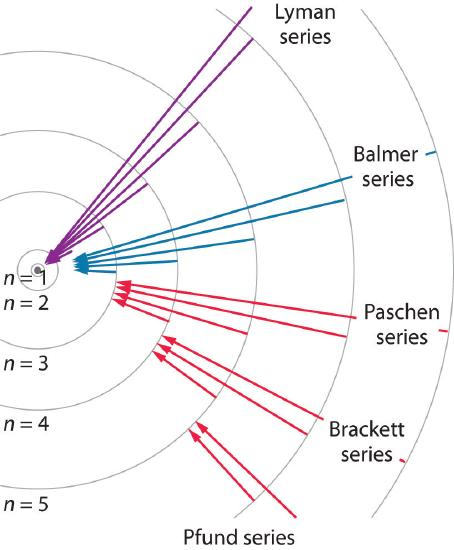
\includegraphics[width=0.6\textwidth,keepaspectratio]{media/hydrogen_emission_series.jpg}
\caption{图 氢原子可见光光谱——氢放电管发出的光经棱镜分光后，在照相底片上记录到一系列分立的谱线（Balmer系）。Hα(656nm)、Hβ(486nm)、Hγ(434nm)、Hδ(410nm)四条特征谱线对应电子在n≥3与n=2之间的跃迁。每一条谱线对应电子在两个定态能级之间的跃迁。}
\end{figure}

氢原子光谱由五组线系组成，每组对应电子跃迁到同一低能级：

{\def\LTcaptype{none} % do not increment counter
\begin{longtable}[]{@{}
  >{\centering\arraybackslash}p{(\linewidth - 6\tabcolsep) * \real{0.2632}}
  >{\centering\arraybackslash}p{(\linewidth - 6\tabcolsep) * \real{0.2632}}
  >{\centering\arraybackslash}p{(\linewidth - 6\tabcolsep) * \real{0.2632}}
  >{\raggedright\arraybackslash}p{(\linewidth - 6\tabcolsep) * \real{0.2105}}@{}}
\toprule\noalign{}
\begin{minipage}[b]{\linewidth}\centering
线系名
\end{minipage} & \begin{minipage}[b]{\linewidth}\centering
低能级 \(n_1\)
\end{minipage} & \begin{minipage}[b]{\linewidth}\centering
光谱区
\end{minipage} & \begin{minipage}[b]{\linewidth}\raggedright
公式
\end{minipage} \\
\midrule\noalign{}
\endhead
\bottomrule\noalign{}
\endlastfoot
Lyman系 & 1 & 紫外 & \(\tilde{\nu} = R_H \left(\frac{1}{1^2} - \frac{1}{n^2}\right)\) \\
\textbf{Balmer系} & \textbf{2} & \textbf{可见光} & \(\tilde{\nu} = R_H \left(\frac{1}{2^2} - \frac{1}{n^2}\right)\) \\
Paschen系 & 3 & 红外 & \(\tilde{\nu} = R_H \left(\frac{1}{3^2} - \frac{1}{n^2}\right)\) \\
Brackett系 & 4 & 红外 & \(\tilde{\nu} = R_H \left(\frac{1}{4^2} - \frac{1}{n^2}\right)\) \\
Pfund系 & 5 & 远红外 & \(\tilde{\nu} = R_H \left(\frac{1}{5^2} - \frac{1}{n^2}\right)\) \\
\end{longtable}
}

其中 Rydberg 常数 \(R_H = 1.097 \times 10^5\ \mathrm{cm^{-1}}\)，\(\tilde{\nu}\) 为波数（单位：\(\mathrm{cm^{-1}}\)）。

\paragraph{② 玻尔的三项革命性假设}\label{ux73bbux5c14ux7684ux4e09ux9879ux9769ux547dux6027ux5047ux8bbe}

Bohr站在Planck量子论（\(E = h\nu\)，能量不连续）、Einstein光子论（\(E = mc^2\)）和Rutherford核式模型的基础上，于1913年提出三项假设：

\textbf{假设一------定态假设}：电子只能在特定半径的轨道上运动，且\textbf{不辐射能量}。这些特殊状态称为''定态''。

\textbf{假设二------角动量量子化}：只有角动量 \(L\) 为 \(h/2\pi\) 整数倍的轨道才是允许的：\(L = n \cdot \dfrac{h}{2\pi}\)，\(n = 1,2,3,\dots\)

\textbf{假设三------跃迁假设}：电子从高能态 \(E_2\) 跃迁到低能态 \(E_1\) 时放出光子：\(\Delta E = E_2 - E_1 = h\nu = hc\tilde{\nu}\)

\paragraph{③ 从假设到公式：玻尔模型的定量推导}\label{ux4eceux5047ux8bbeux5230ux516cux5f0fux73bbux5c14ux6a21ux578bux7684ux5b9aux91cfux63a8ux5bfc}

由假设二（角动量量子化）和经典力学（库仑力 = 向心力）可导出轨道半径和能量：

\[
\begin{aligned}
\text{库仑力} &: \quad \frac{e^2}{4\pi\varepsilon_0 r^2} = \frac{mv^2}{r} \\
\text{角动量量子化} &: \quad mvr = n\frac{h}{2\pi}
\end{aligned}
\]

联立消去 \(v\)，解得轨道半径：

\[
r_n = \frac{\varepsilon_0 h^2}{\pi m e^2} \cdot n^2 = a_0 \cdot n^2
\]

其中 \(a_0 = 52.9\ \mathrm{pm}\) 称为\textbf{Bohr半径}。

电子能量 = 动能 + 势能：

\[
E_n = \frac{1}{2}mv^2 - \frac{e^2}{4\pi\varepsilon_0 r} = -\frac{e^2}{8\pi\varepsilon_0 r} = -\frac{me^4}{8\varepsilon_0^2 h^2} \cdot \frac{1}{n^2}
\]

代入常数得：

\[
\boxed{E_n = -\frac{13.6}{n^2}\ \mathrm{eV}}
\]

\paragraph{④ 成功与局限：为什么玻尔模型重要但又不够？}\label{ux6210ux529fux4e0eux5c40ux9650ux4e3aux4ec0ux4e48ux73bbux5c14ux6a21ux578bux91cdux8981ux4f46ux53c8ux4e0dux591f}

\textbf{成功}：
- 完美预测氢原子光谱五线系（Balmer系\(H_\alpha\)线：656.3 nm，与实验吻合）
- 计算了Bohr半径 \(a_0 = 52.9\ \mathrm{pm}\) 和基态能量 \(-13.6\ \mathrm{eV}\)
- 预测氢原子电离能 \(I = 13.6\ \mathrm{eV} = 1.31 \times 10^3\ \mathrm{kJ\cdot mol^{-1}}\)
- 可推广至类氢离子（\(\mathrm{He^+, Li^{2+}}\)）------只需将 \(e^2\) 换为 \(Ze^2\)：

\[E_n = -13.6 \cdot \frac{Z^2}{n^2}\ \mathrm{eV}\]

\textbf{局限}：
- ❌ 不能解释氢原子光谱精细结构（每一条谱线实际上分裂为两条）
- ❌ 不能解释多电子原子（He即出现显著偏差------因忽略了电子-电子排斥）
- ❌ 定态假设本身与经典电磁理论相悖（为什么电子加速但不辐射？）
- ❌ 无法解释Zeeman效应（磁场中谱线分裂）

\textbf{关键启示}：``轨道''（orbit）概念在此走到尽头。玻尔模型是旧量子论的巅峰，但它保留了太多经典物理的痕迹。真正的突破需要放弃''电子有确定位置''这一前提------这正是下一节的主题。

\begin{quote}
💡 \textbf{深层理解}：「玻尔模型虽然不完整，但它的成功揭示了经典物理在原子尺度的边界------电子不像行星绕太阳那样沿固定轨道运动。它引入了量子化这一核心思想，只是还不够彻底。」
\end{quote}

📌 \textbf{理解要点}：``波尔模型能解释氢原子光谱------但它说电子有轨道。轨道这个概念本身是错的。电子没有确定的轨道------只有概率密度。从玻尔到量子力学------是放弃'轨道'、接受'概率云'的思维升级。''

\paragraph{\texorpdfstring{⑤ 练习：Balmer系\(H_\alpha\)线波长}{⑤ 练习：Balmer系H\_\textbackslash alpha线波长}}\label{ux7ec3ux4e60balmerux7cfbh_alphaux7ebfux6ce2ux957f}

\textbf{题目}：\(H_\alpha\)线对应电子从 \(n=3\) 跃迁到 \(n=2\)。已知 \(R_H = 1.097 \times 10^5\ \mathrm{cm^{-1}}\)，计算\(H_\alpha\)线的波长（nm）。

\textbf{解答}：

\[
\tilde{\nu} = 1.097\times 10^5 \times \left(\frac{1}{4} - \frac{1}{9}\right) = 1.097\times 10^5 \times \frac{5}{36} = 15236\ \mathrm{cm^{-1}}
\]

\[
\lambda = \frac{1}{\tilde{\nu}} = \frac{1}{15236}\ \mathrm{cm} = 6.563\times 10^{-5}\ \mathrm{cm} = 656.3\ \mathrm{nm}
\]

\textbf{验证}：656.3 nm对应可见光红色------与实验观测的\(H_\alpha\)红线完全一致。

------

\subsubsection{1.3 波粒二象性与测不准原理：经典''轨道''概念的终结}\label{ux6ce2ux7c92ux4e8cux8c61ux6027ux4e0eux6d4bux4e0dux51c6ux539fux7406ux7ecfux5178ux8f68ux9053ux6982ux5ff5ux7684ux7ec8ux7ed3}

\paragraph{① 德布罗意的天才猜想}\label{ux5fb7ux5e03ux7f57ux610fux7684ux5929ux624dux731cux60f3}

1924年，法国物理学家Louis de Broglie在他的博士论文中提出一个革命性假设：\textbf{不仅光具有波粒二象性，所有实物粒子（电子、质子、中子、原子）也都具有波动性}。

\[\lambda = \frac{h}{p} = \frac{h}{mv}\]

\textbf{直观理解}：粒子的质量越大、速度越快，波长越短，波动性越不明显。宏观物体的波长小到无法观测（一枚10g子弹以300 m/s运动的 \(\lambda \approx 2\times 10^{-34}\ \mathrm{m}\)------比原子核还小数亿倍）。但电子的质量极小（\(9.109\times 10^{-31}\ \mathrm{kg}\)），在原子尺度下的波长与原子大小相当------\textbf{波动性不可忽略}。

\textbf{实验验证}：1927年，Davisson和Germer在晶体表面观察到电子的衍射现象------与X射线衍射类似，电子在Ni晶体表面产生了清晰的衍射条纹。这直接证明了电子的波动性。

\textbf{💡 量化感知：不同粒子的 de Broglie 波长}

下面这张表来自普化原理，把不同粒子的波长放在一起对比------可以直观地看到：

{\def\LTcaptype{none} % do not increment counter
\begin{longtable}[]{@{}
  >{\raggedright\arraybackslash}p{(\linewidth - 6\tabcolsep) * \real{0.2222}}
  >{\raggedleft\arraybackslash}p{(\linewidth - 6\tabcolsep) * \real{0.2222}}
  >{\centering\arraybackslash}p{(\linewidth - 6\tabcolsep) * \real{0.2778}}
  >{\centering\arraybackslash}p{(\linewidth - 6\tabcolsep) * \real{0.2778}}@{}}
\toprule\noalign{}
\begin{minipage}[b]{\linewidth}\raggedright
粒子
\end{minipage} & \begin{minipage}[b]{\linewidth}\raggedleft
质量 m/kg
\end{minipage} & \begin{minipage}[b]{\linewidth}\centering
速度 v/(m·s\textsuperscript{-1})
\end{minipage} & \begin{minipage}[b]{\linewidth}\centering
波长 λ/pm
\end{minipage} \\
\midrule\noalign{}
\endhead
\bottomrule\noalign{}
\endlastfoot
1V 加速电子 & \(9.1\times 10^{-31}\) & \(5.9\times 10^5\) & \(1.2\times 10^{3}\) \\
100V 加速电子 & \(9.1\times 10^{-31}\) & \(5.9\times 10^6\) & \(1.2\times 10^{2}\) \\
1000V 加速电子 & \(9.1\times 10^{-31}\) & \(1.9\times 10^7\) & \(37\) \\
10000V 加速电子 & \(9.1\times 10^{-31}\) & \(5.9\times 10^7\) & \(12\) \\
He 原子（300 K） & \(6.6\times 10^{-27}\) & \(1.4\times 10^3\) & \(72\) \\
Xe 原子（300 K） & \(2.3\times 10^{-25}\) & \(2.4\times 10^2\) & \(12\) \\
垒球 & \(2.0\times 10^{-1}\) & \(30\) & \(1.1\times 10^{-22}\) \\
枪弹 & \(1.0\times 10^{-2}\) & \(1.0\times 10^3\) & \(6.6\times 10^{-23}\) \\
\end{longtable}
}

\textbf{解读}：电子和稀有气体原子的波长与 X 射线相当（\(\sim 10\text{–}10^3\) pm），可通过晶体衍射观测其波动性。而宏观物体（垒球、枪弹）的波长比原子核还小数十亿倍------完全无法测量。\textbf{波动性不是宏观物体没有，而是小到可以忽略}。这也是为什么经典力学对宏观物体成立------因为 Planck 常数 \(h\) 太小，量子效应在宏观尺度被压制。

\paragraph{② 海森堡测不准原理}\label{ux6d77ux68eeux5821ux6d4bux4e0dux51c6ux539fux7406}

既然电子具有波动性，就不可能同时精确测定它的位置和动量。1927年，Heisenberg提出了测不准原理的定量表达式：

\[
\boxed{\Delta x \cdot \Delta p \geq \frac{h}{4\pi}}
\]

\paragraph{③ 练习：为什么原子中不存在电子''轨道''？}\label{ux7ec3ux4e60ux4e3aux4ec0ux4e48ux539fux5b50ux4e2dux4e0dux5b58ux5728ux7535ux5b50ux8f68ux9053}

\textbf{题目}：电子在原子中的运动范围约 \(r \approx 10^{-10}\ \mathrm{m}\)。若位置误差 \(\Delta x = 10^{-10}\ \mathrm{m}\)，计算电子速度的不确定度 \(\Delta v\)。

\textbf{解答}：

由测不准原理：

\[\Delta p \geq \frac{h}{4\pi \cdot \Delta x} = \frac{6.626\times 10^{-34}}{4\pi \times 10^{-10}} \approx 5.27\times 10^{-25}\ \mathrm{kg\cdot m/s}\]

\[\Delta v \geq \frac{\Delta p}{m_e} = \frac{5.27\times 10^{-25}}{9.109\times 10^{-31}} \approx 5.8\times 10^5\ \mathrm{m/s}\]

\textbf{结论}：\(\Delta v \approx 5.8\times 10^5\ \mathrm{m/s}\)，与电子在原子中的运动速度（\(\sim 10^6\ \mathrm{m/s}\)）\textbf{同一量级}。这意味着我们完全无法确定电子''在轨道上某点的速度''------\textbf{``轨道''概念在原子尺度失去了意义}。

\begin{quote}
💡 \textbf{通俗理解}：「你想看电子在哪儿------用光子照它。但光子有动量------一照就把电子踢走了。测得越精确（Δx小）→光子波长越短→动量越大→Δp越大。你永远不能同时精确知道位置和动量。」
\end{quote}

\paragraph{④ 从''轨道''到''概率''}\label{ux4eceux8f68ux9053ux5230ux6982ux7387}

既然没有确定的轨道，电子该怎么描述？

1926年，奥地利物理学家Erwin Schrödinger提出了波动方程------\textbf{薛定谔方程}，以波函数 \(\psi\)（读作''赛''）来描述电子的运动状态。\(\psi\) 本身是\textbf{概率振幅}，而 \(\|\psi\|^2\) 表示电子在空间某点出现的\textbf{概率密度}。

\textbf{电子云}就是 \(\|\psi\|^2\) 的可视化------黑点密集的地方，电子出现的概率大；稀疏的地方，概率小。这不是云，是概率的散布图。

------

\subsection{二、核外电子运动状态的描述}\label{ux4e8cux6838ux5916ux7535ux5b50ux8fd0ux52a8ux72b6ux6001ux7684ux63cfux8ff0}

\textbf{关联知识点}：量子数 · 原子轨道 · 屏蔽效应 · 钻穿效应

\subsubsection{2.1 薛定谔方程与三个量子数的自然出现}\label{ux859bux5b9aux8c14ux65b9ux7a0bux4e0eux4e09ux4e2aux91cfux5b50ux6570ux7684ux81eaux7136ux51faux73b0}

\paragraph{① 薛定谔方程}\label{ux859bux5b9aux8c14ux65b9ux7a0b}

对于一个质量为 \(m\)、在势能为 \(V\) 的势场中运动的电子，其运动状态由以下方程描述：

\[
\boxed{\frac{\partial^2 \psi}{\partial x^2} + \frac{\partial^2 \psi}{\partial y^2} + \frac{\partial^2 \psi}{\partial z^2} + \frac{8\pi^2 m}{h^2}(E - V)\psi = 0}
\]

\paragraph{② 坐标变换：从直角坐标到球极坐标}\label{ux5750ux6807ux53d8ux6362ux4eceux76f4ux89d2ux5750ux6807ux5230ux7403ux6781ux5750ux6807}

由于原子具有\textbf{球对称性}，将Schrödinger方程从直角坐标 \((x,y,z)\) 变换到球极坐标 \((r,\theta,\varphi)\)：

\begin{figure}[H]\centering
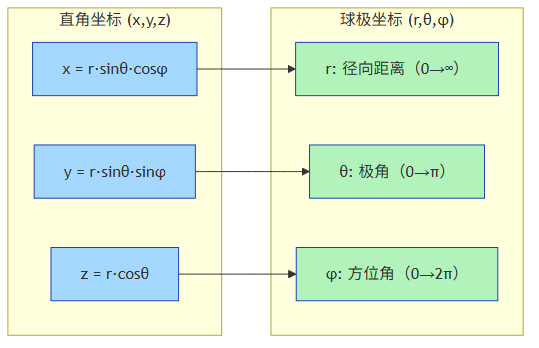
\includegraphics[width=0.45\textwidth,keepaspectratio]{media/excalidraw-原子结构-schrodinger-coordinate-transform.png}
\caption{图 直角坐标与球极坐标变换关系图——从(x,y,z)到(r,θ,φ)的变换：x = r sinθ cosφ, y = r sinθ sinφ, z = r cosθ}
\end{figure}

\textbf{口诀}：\(r\) 是到原点的距离，\(\theta\) 是跟 z 轴夹角，\(\varphi\) 是绕 z 轴转过的角度。

\[
\begin{aligned}
x &= r\sin\theta\cos\varphi \\[2pt]
y &= r\sin\theta\sin\varphi \\[2pt]
z &= r\cos\theta
\end{aligned}
\]

\textbf{球极坐标下的Schrödinger方程}（了解即可，不需记忆）：

\[
\left[\frac{1}{r^2}\frac{\partial}{\partial r}\left(r^2\frac{\partial}{\partial r}\right) + \frac{1}{r^2\sin\theta}\frac{\partial}{\partial\theta}\left(\sin\theta\frac{\partial}{\partial\theta}\right) + \frac{1}{r^2\sin^2\theta}\frac{\partial^2}{\partial\varphi^2}\right]\psi + \frac{8\pi^2 m}{h^2}\left(E - \frac{Ze^2}{r}\right)\psi = 0
\]

\paragraph{③ 变量分离与量子数的引入}\label{ux53d8ux91cfux5206ux79bbux4e0eux91cfux5b50ux6570ux7684ux5f15ux5165}

通过\textbf{变量分离法}，将 \(\psi\) 分解为径向部分和角度部分：

\[
\boxed{\psi_{n,l,m}(r,\theta,\varphi) = R_{n,l}(r) \cdot Y_{l,m}(\theta,\varphi)}
\]

{\def\LTcaptype{none} % do not increment counter
\begin{longtable}[]{@{}
  >{\centering\arraybackslash}p{(\linewidth - 8\tabcolsep) * \real{0.2174}}
  >{\centering\arraybackslash}p{(\linewidth - 8\tabcolsep) * \real{0.2174}}
  >{\raggedright\arraybackslash}p{(\linewidth - 8\tabcolsep) * \real{0.1739}}
  >{\centering\arraybackslash}p{(\linewidth - 8\tabcolsep) * \real{0.2174}}
  >{\raggedright\arraybackslash}p{(\linewidth - 8\tabcolsep) * \real{0.1739}}@{}}
\toprule\noalign{}
\begin{minipage}[b]{\linewidth}\centering
量子数
\end{minipage} & \begin{minipage}[b]{\linewidth}\centering
符号
\end{minipage} & \begin{minipage}[b]{\linewidth}\raggedright
来源
\end{minipage} & \begin{minipage}[b]{\linewidth}\centering
取值范围
\end{minipage} & \begin{minipage}[b]{\linewidth}\raggedright
决定的物理量
\end{minipage} \\
\midrule\noalign{}
\endhead
\bottomrule\noalign{}
\endlastfoot
\textbf{主量子数} & \(n\) & 径向方程边界条件 & 1, 2, 3, \ldots{} & 电子层、主要能量 \\
\textbf{角量子数} & \(l\) & 角度方程边界条件 & 0, 1, \ldots, \(n-1\) & 轨道形状、能级分裂 \\
\textbf{磁量子数} & \(m_l\) & 角度方程边界条件 & \(-l, ..., 0, ..., +l\) & 轨道空间取向 \\
\end{longtable}
}

\textbf{关键认识}：量子数不是人为假定的，而是边界条件迫使 \(n,l,m\) 只能取特定整数值------这是量子力学的\textbf{自然推论}。

------

\subsubsection{2.2 四个量子数的详细解读}\label{ux56dbux4e2aux91cfux5b50ux6570ux7684ux8be6ux7ec6ux89e3ux8bfb}

\paragraph{\texorpdfstring{（1）主量子数 \(n\)------电子层}{（1）主量子数 n------电子层}}\label{ux4e3bux91cfux5b50ux6570-nux7535ux5b50ux5c42}

{\def\LTcaptype{none} % do not increment counter
\begin{longtable}[]{@{}lccccccc@{}}
\toprule\noalign{}
\(n\) 取值 & 1 & 2 & 3 & 4 & 5 & 6 & 7 \\
\midrule\noalign{}
\endhead
\bottomrule\noalign{}
\endlastfoot
能层符号 & \textbf{K} & \textbf{L} & \textbf{M} & \textbf{N} & \textbf{O} & \textbf{P} & \textbf{Q} \\
\end{longtable}
}

\begin{itemize}
\tightlist
\item
  单电子体系：\(E_n = -13.6 Z^2/n^2\ \mathrm{eV}\)
\item
  \(n\) 越大，电子离核越远，能量越高，原子半径越大
\item
  轨道总数 \(n^2\)，最大电子数 \(2n^2\)
\end{itemize}

\paragraph{\texorpdfstring{（2）角量子数 \(l\)------轨道形状}{（2）角量子数 l------轨道形状}}\label{ux89d2ux91cfux5b50ux6570-lux8f68ux9053ux5f62ux72b6}

{\def\LTcaptype{none} % do not increment counter
\begin{longtable}[]{@{}ccccccc@{}}
\toprule\noalign{}
\(l\) 取值 & 0 & 1 & 2 & 3 & 4 & 5 \\
\midrule\noalign{}
\endhead
\bottomrule\noalign{}
\endlastfoot
能级符号 & \textbf{s} & \textbf{p} & \textbf{d} & \textbf{f} & \textbf{g} & \textbf{h} \\
轨道形状 & \textbf{球形} & \textbf{哑铃形} & \textbf{花瓣形} & 复杂 & 复杂 & 复杂 \\
\end{longtable}
}

\begin{itemize}
\tightlist
\item
  在多电子原子中，\(l\) 与 \(n\) \textbf{共同决定}电子能量
\item
  节面数 = \(l\)
\end{itemize}

\begin{figure}[H]\centering
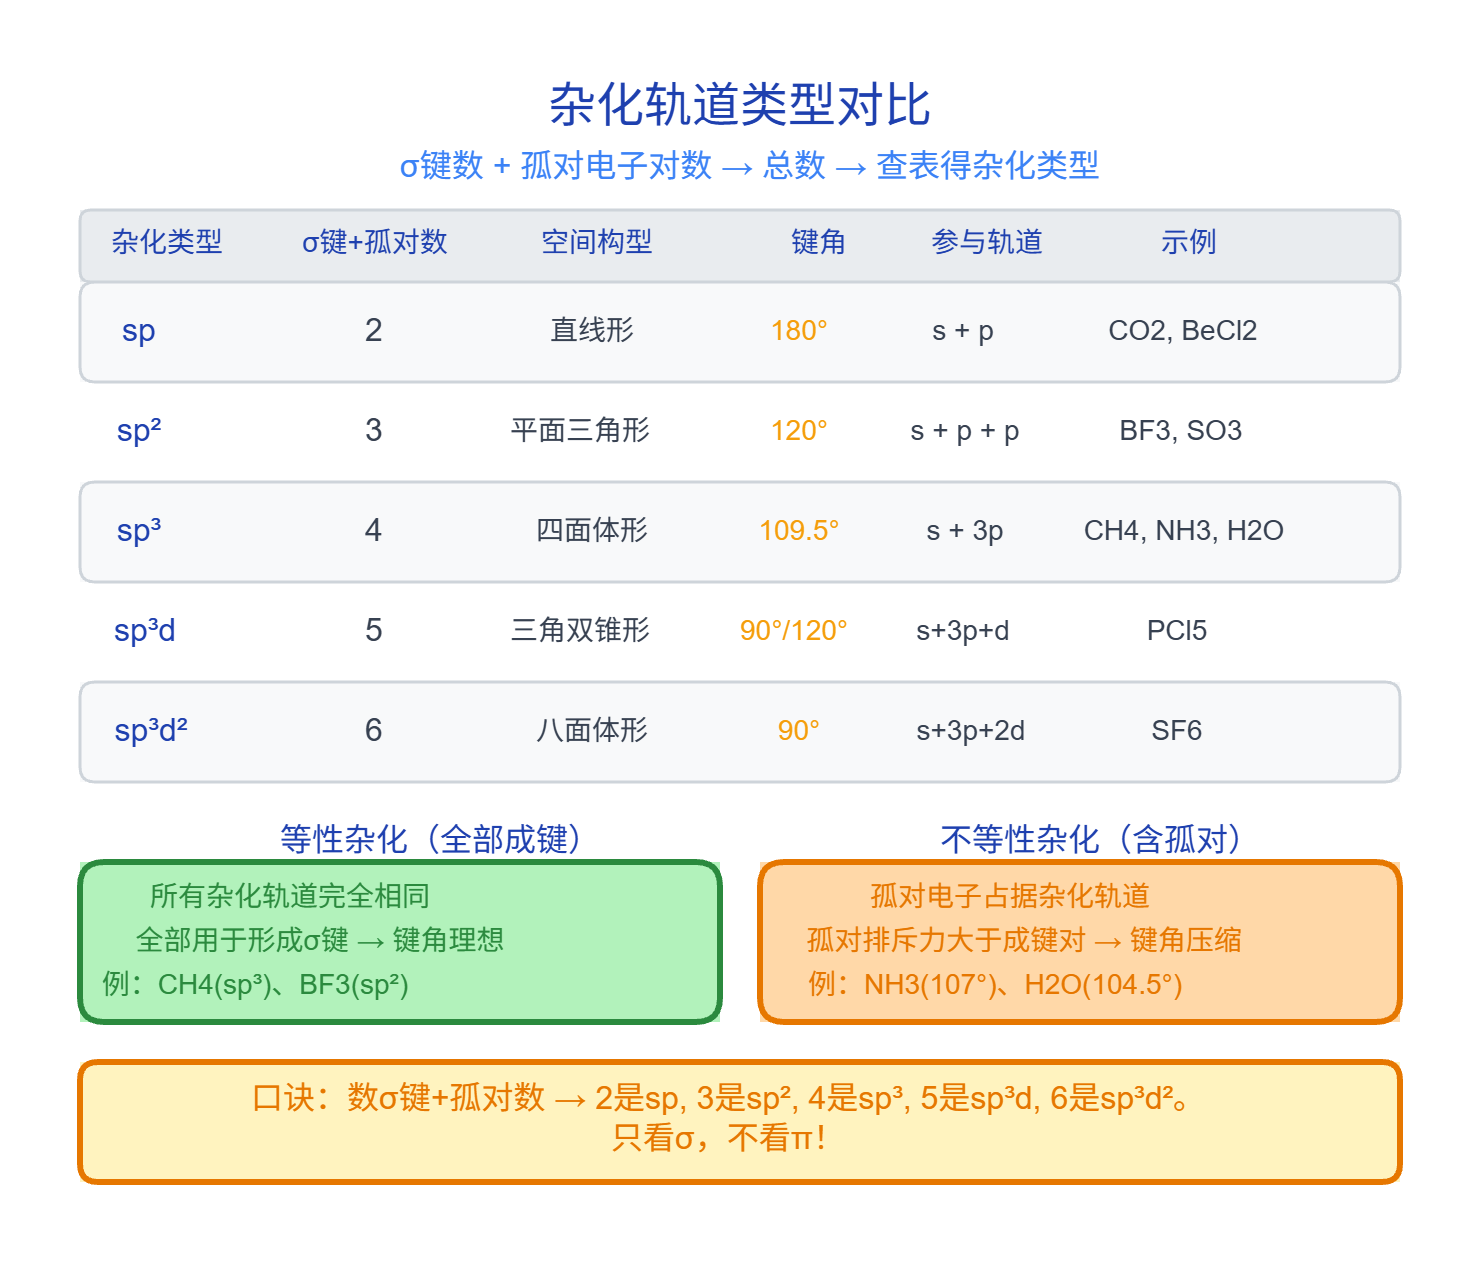
\includegraphics[width=0.45\textwidth,keepaspectratio]{media/11-13-orbital-shapes-s-p-d.jpg}
\caption{图 s、p、d 轨道角度分布图——s球形，p哑铃形，d花瓣形（普化原理第4版 图11.13）}
\end{figure}

\begin{figure}[H]\centering
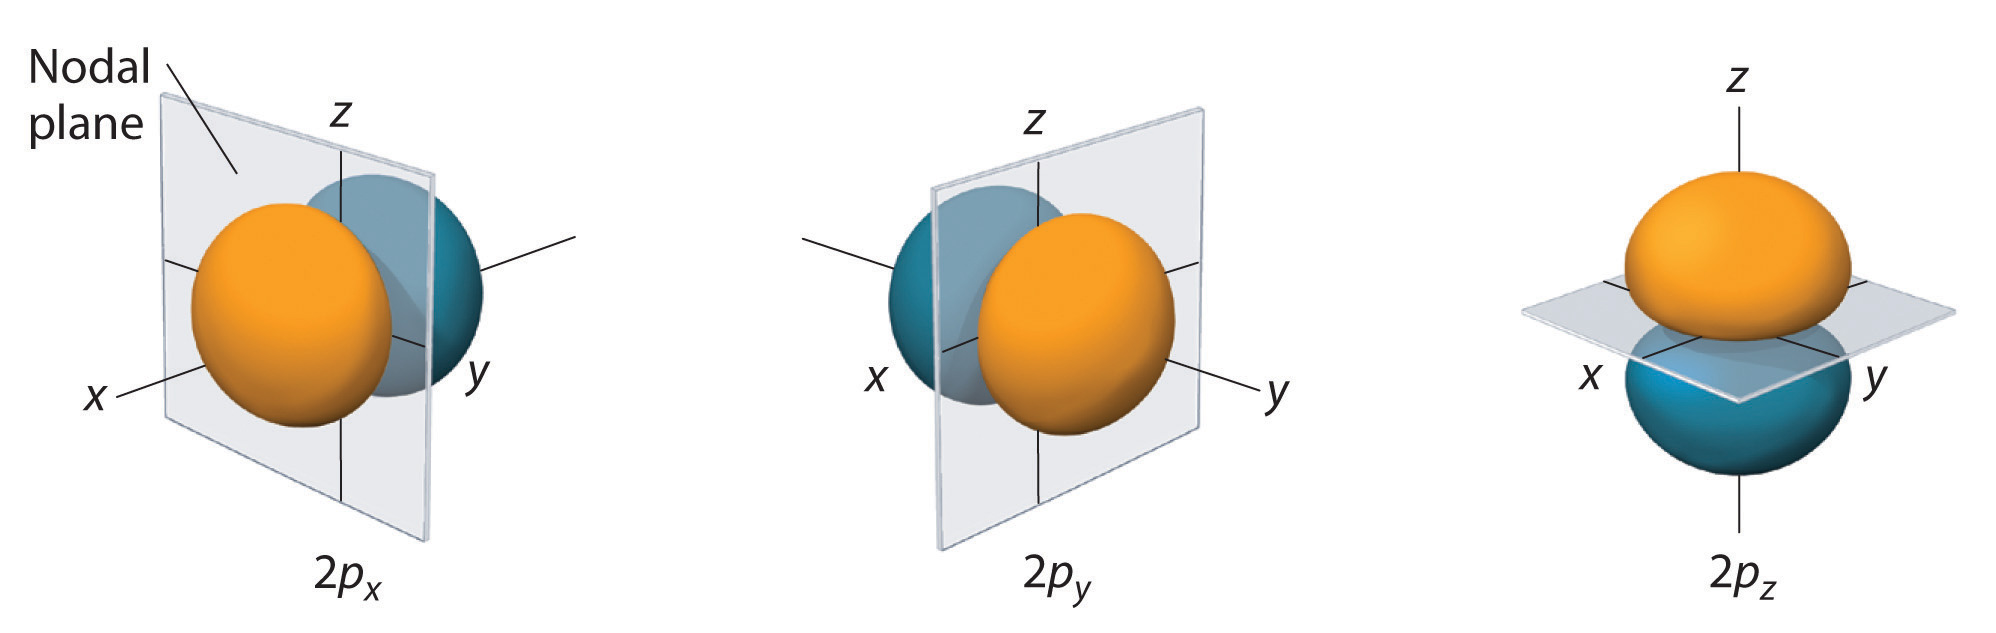
\includegraphics[width=0.45\textwidth,keepaspectratio]{media/orbital_2p_three_orientations.jpg}
\caption{图 p轨道的三维形状与空间取向——p轨道呈哑铃形，分别沿x、y、z轴方向伸展，节面通过原子核。（普化原理第4版）}
\end{figure}

\begin{figure}[H]\centering
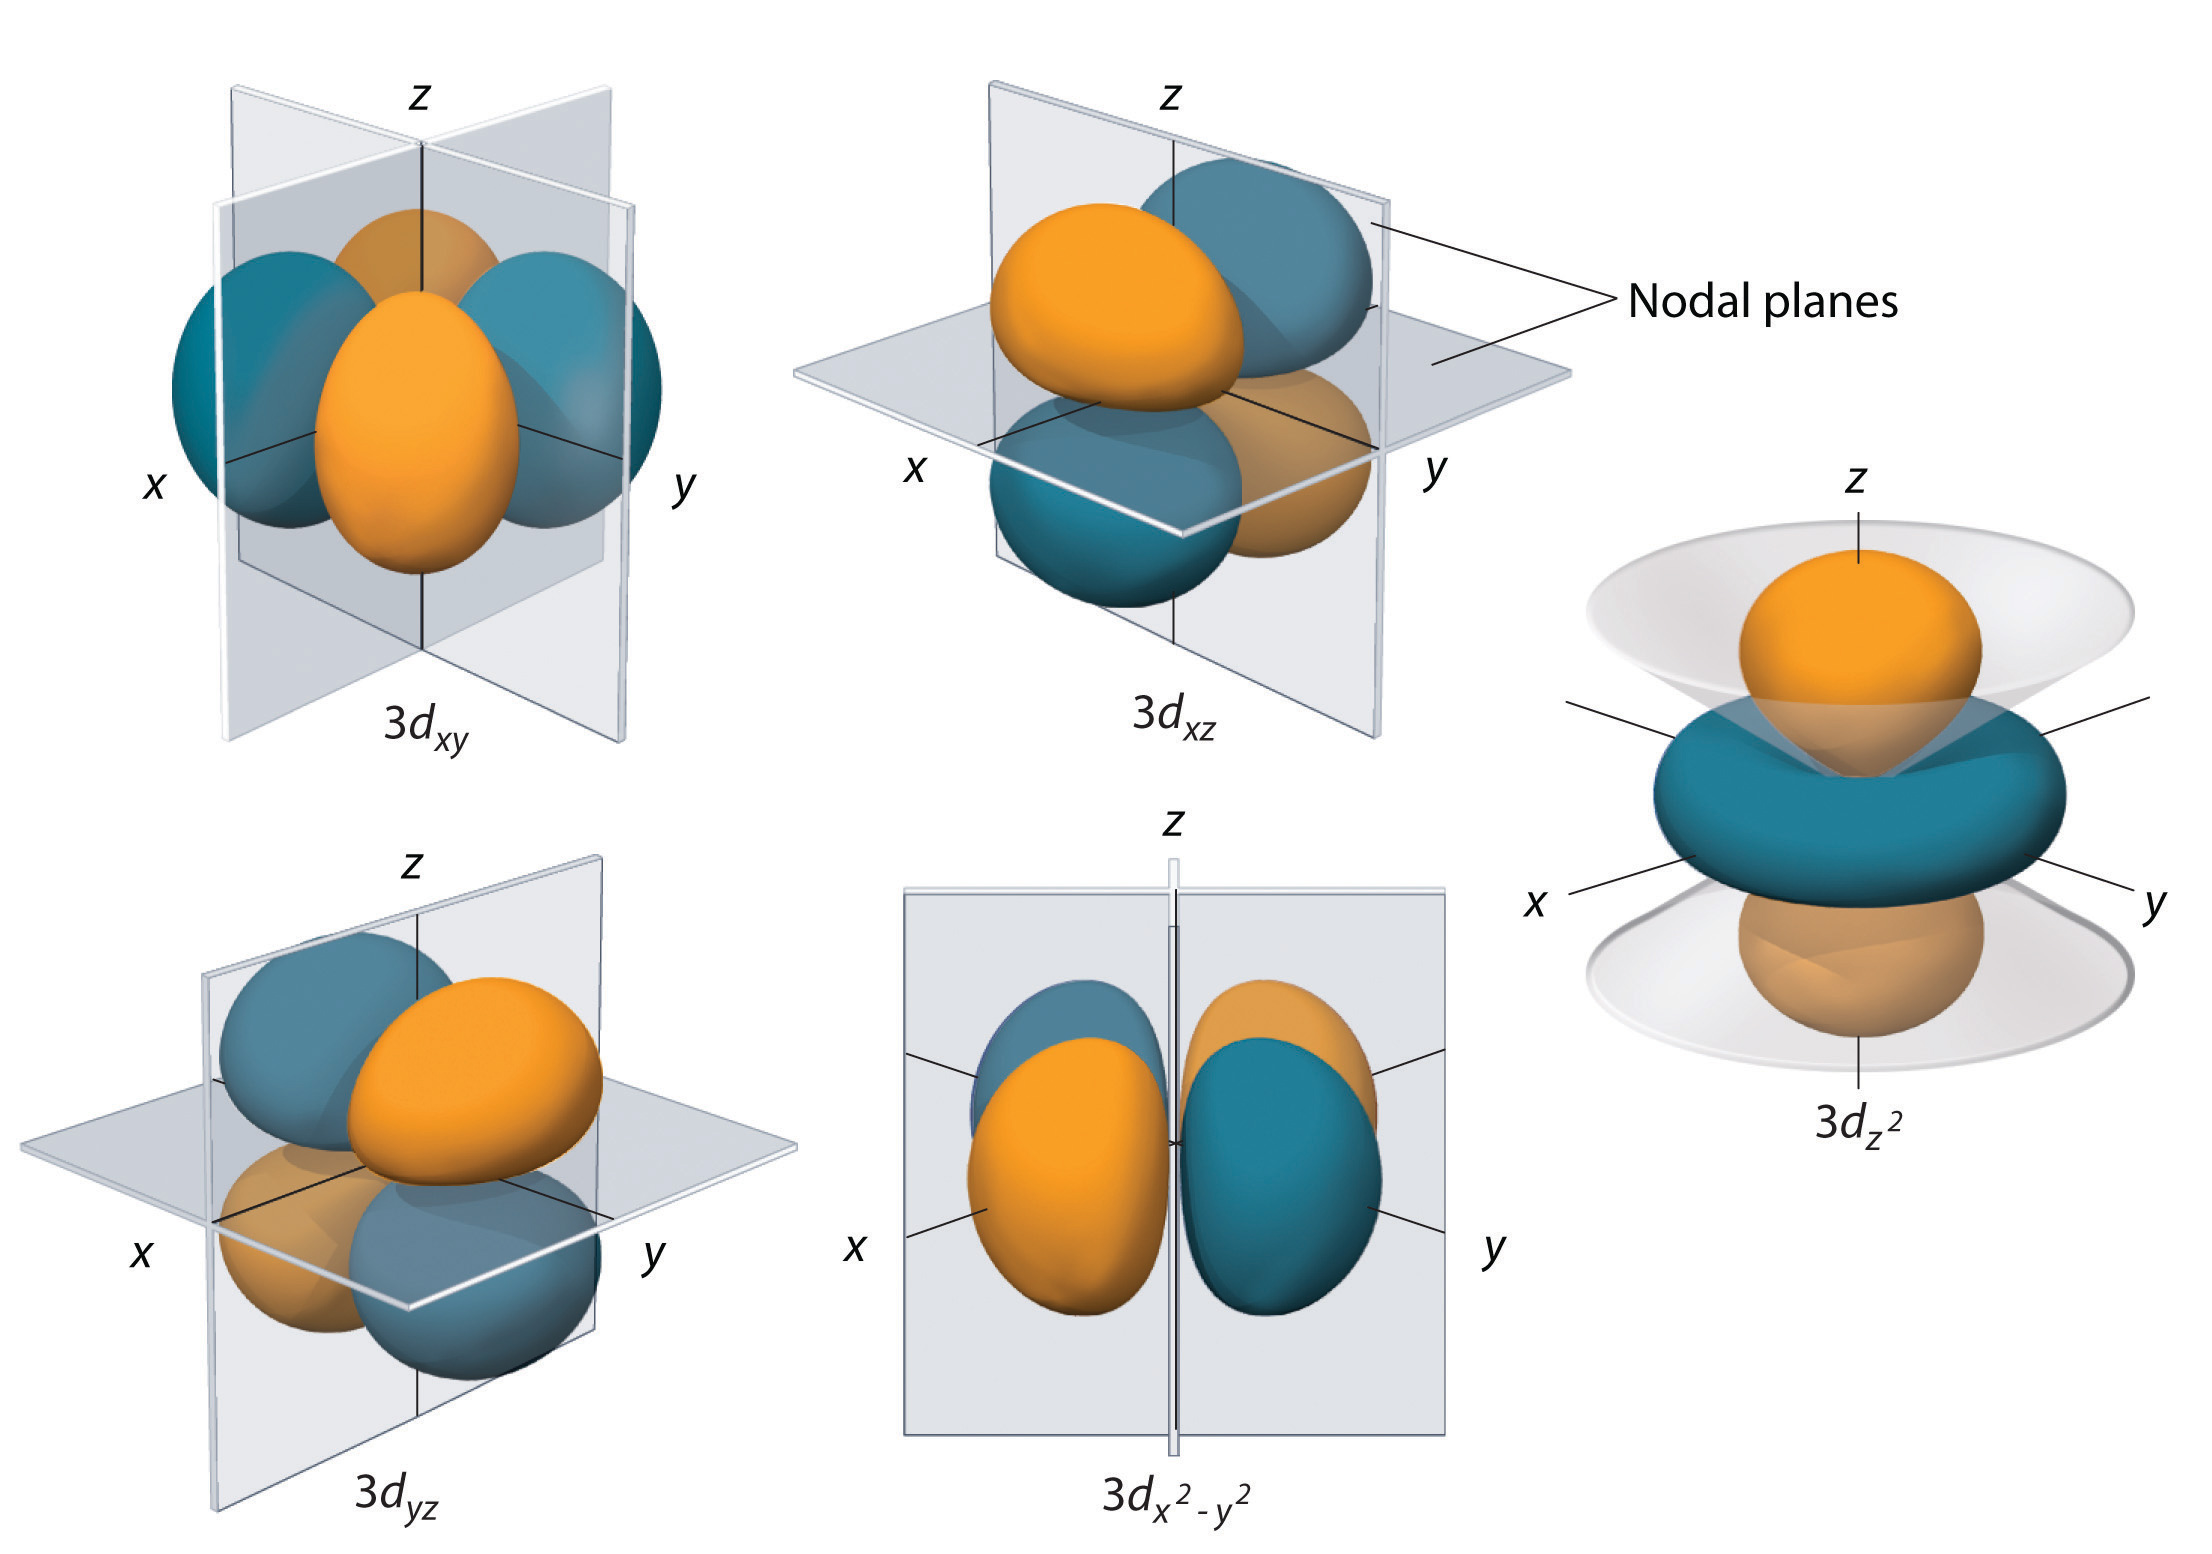
\includegraphics[width=0.45\textwidth,keepaspectratio]{media/orbital_3d_five_orientations.jpg}
\caption{图 d轨道的三维形状与空间取向——五个d轨道中dxy、dxz、dyz、dx2-y2呈四瓣形，dz2呈两瓣加环形区。节面数=2。（普化原理第4版）}
\end{figure}

\textbf{径向分布函数 \(D(r)\) 的引入}
上一节通过变量分离得到 \(\psi_{n,l,m}(r,\theta,\varphi)=R_{n,l}(r)Y_{l,m}(\theta,\varphi)\)。其中角度部分 \(Y_{l,m}\) 决定了轨道的空间取向（即上图中的形状），而径向部分 \(R_{n,l}(r)\) 决定了电子在距核不同距离处出现的概率。将 \(\|\psi\|^2\) 对全部角度 \((\theta,\varphi)\) 积分，消去角度依赖，得到仅关于径向距离 \(r\) 的\textbf{径向分布函数}：
\[D_{n,l}(r) = 4\pi r^2 |R_{n,l}(r)|^2\]
\(D(r)dr\) 表示电子出现在距核 \(r\) 到 \(r+dr\) 球壳内的概率。\(D(r)\) 对 \(r\) 作图即\textbf{径向概率分布图}，它是理解钻穿效应、屏蔽效应和能级分裂的定量基础。

\begin{figure}[H]\centering
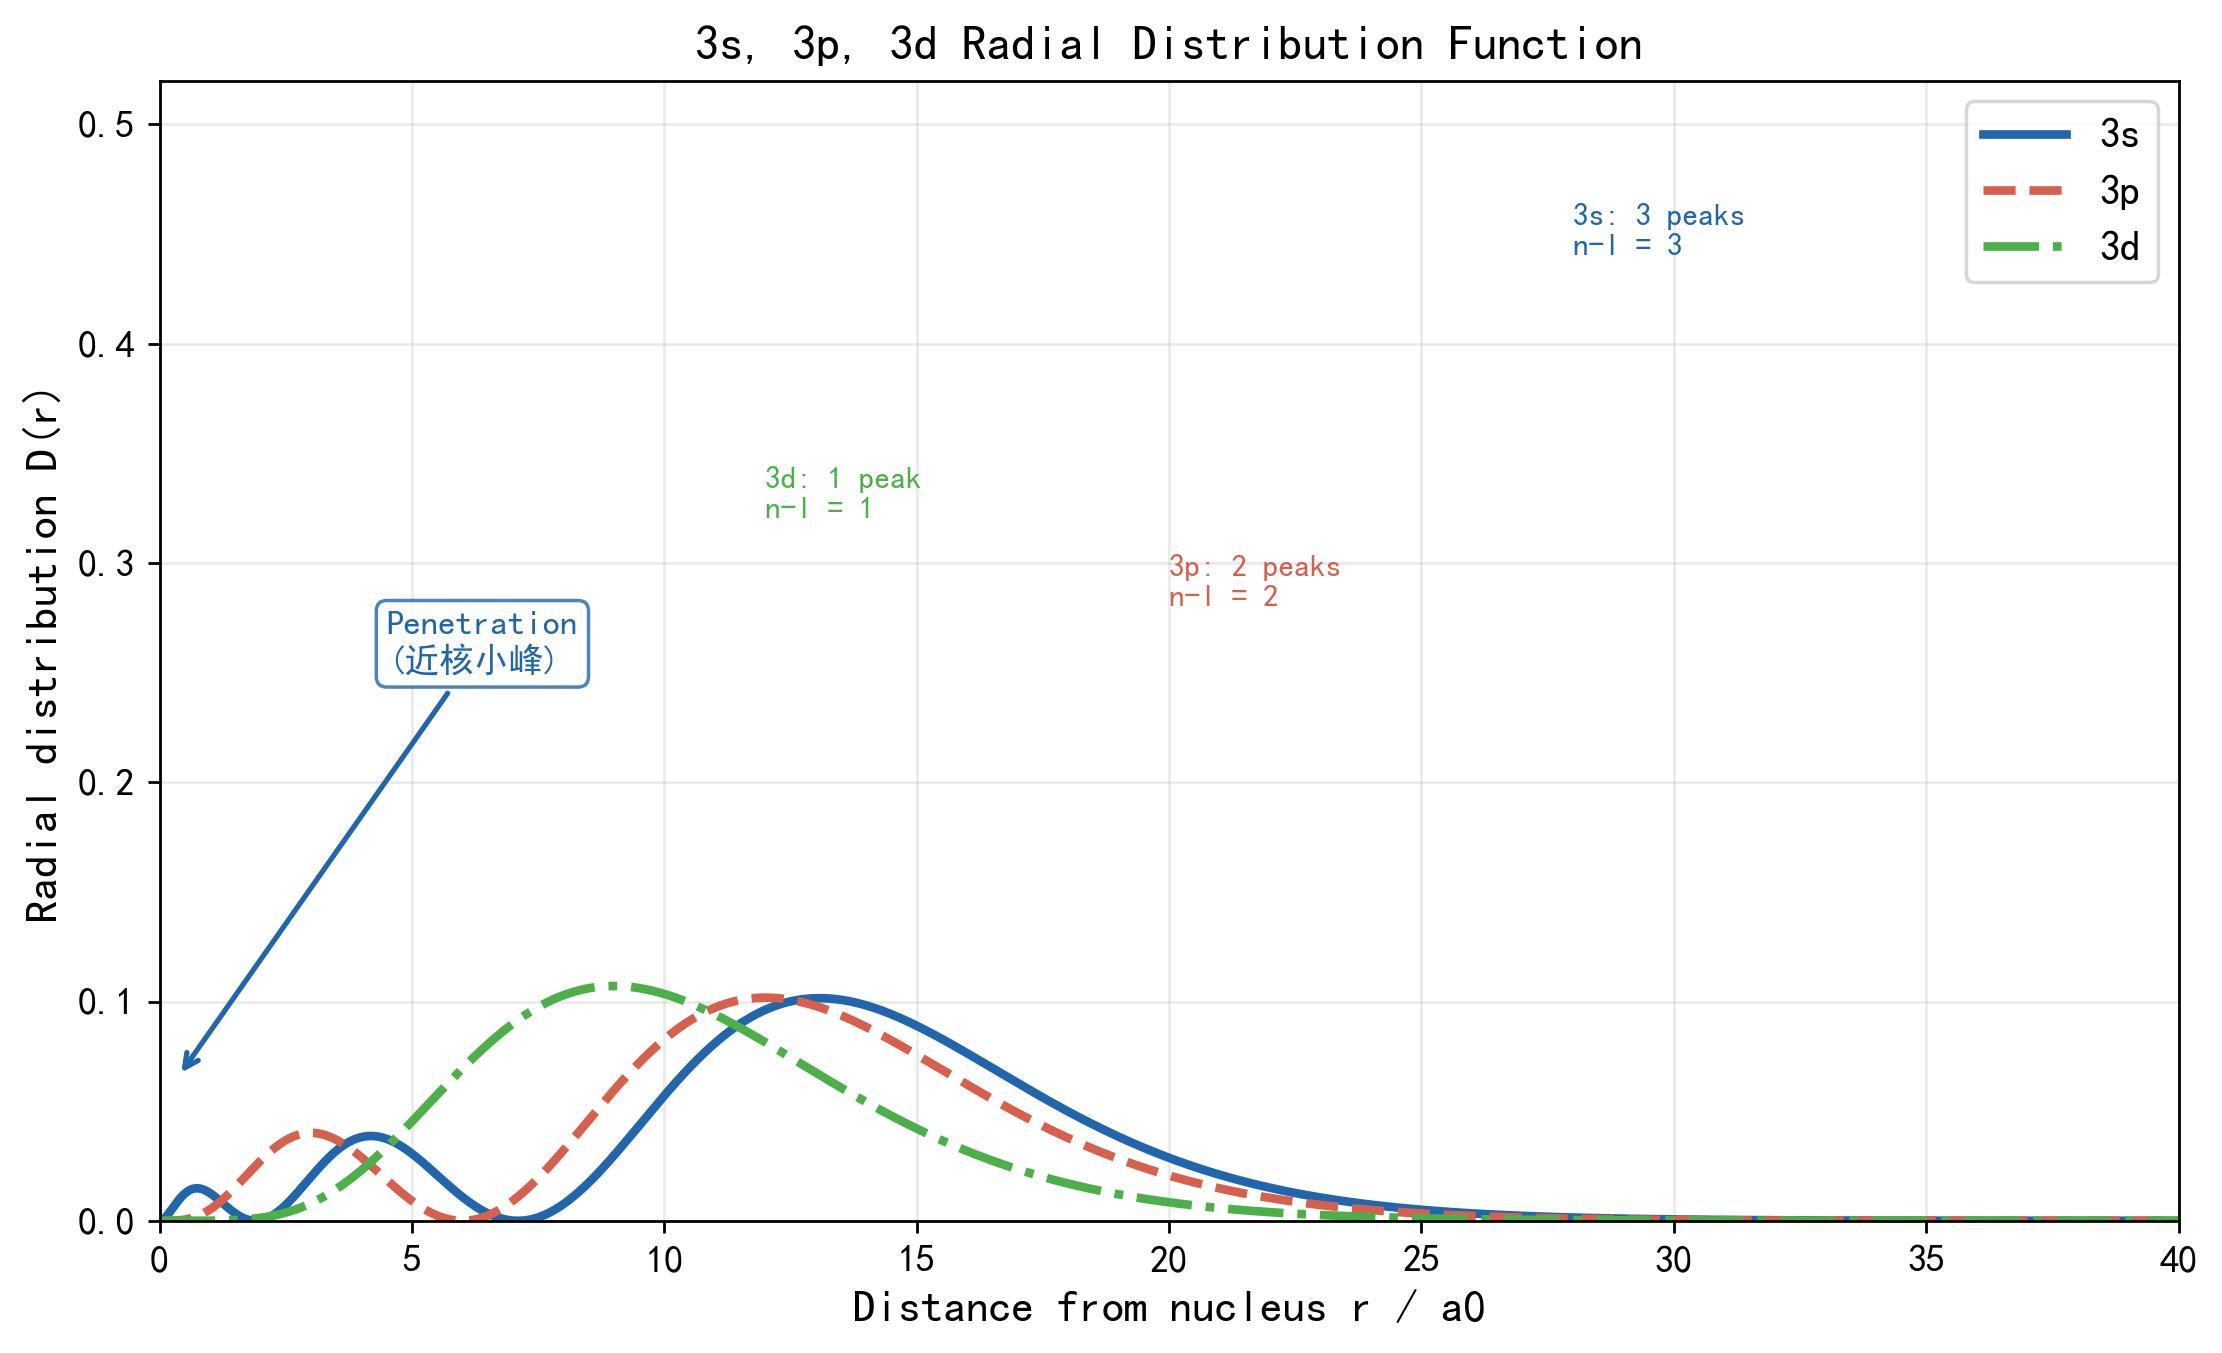
\includegraphics[width=0.45\textwidth,keepaspectratio]{media/11-21-radial-distribution-3s-3p-3d.jpg}
\caption{图 3s、3p、3d径向分布函数 D(r) 对比——3s有三个峰（n-l=3，含近核小峰），3p有两个峰，3d有一个峰。横轴为距核距离 r，纵轴为径向概率密度。最外峰位置反映轨道”半径”大小。近核区域仅s轨道有小峰——这是钻穿效应的直接体现。（普化原理第4版 图11.21）}
\end{figure}

\textbf{从径向分布看钻穿效应}
比较上图3s、3p、3d的 \(D(r)\) 曲线：s轨道（\(l=0\)）在近核处有\textbf{小峰}（钻穿到内层），感受更大的有效核电荷 \(Z^*\)，因此能量比同层p、d更低。这正是能级分裂的物理根源。

\begin{figure}[H]\centering
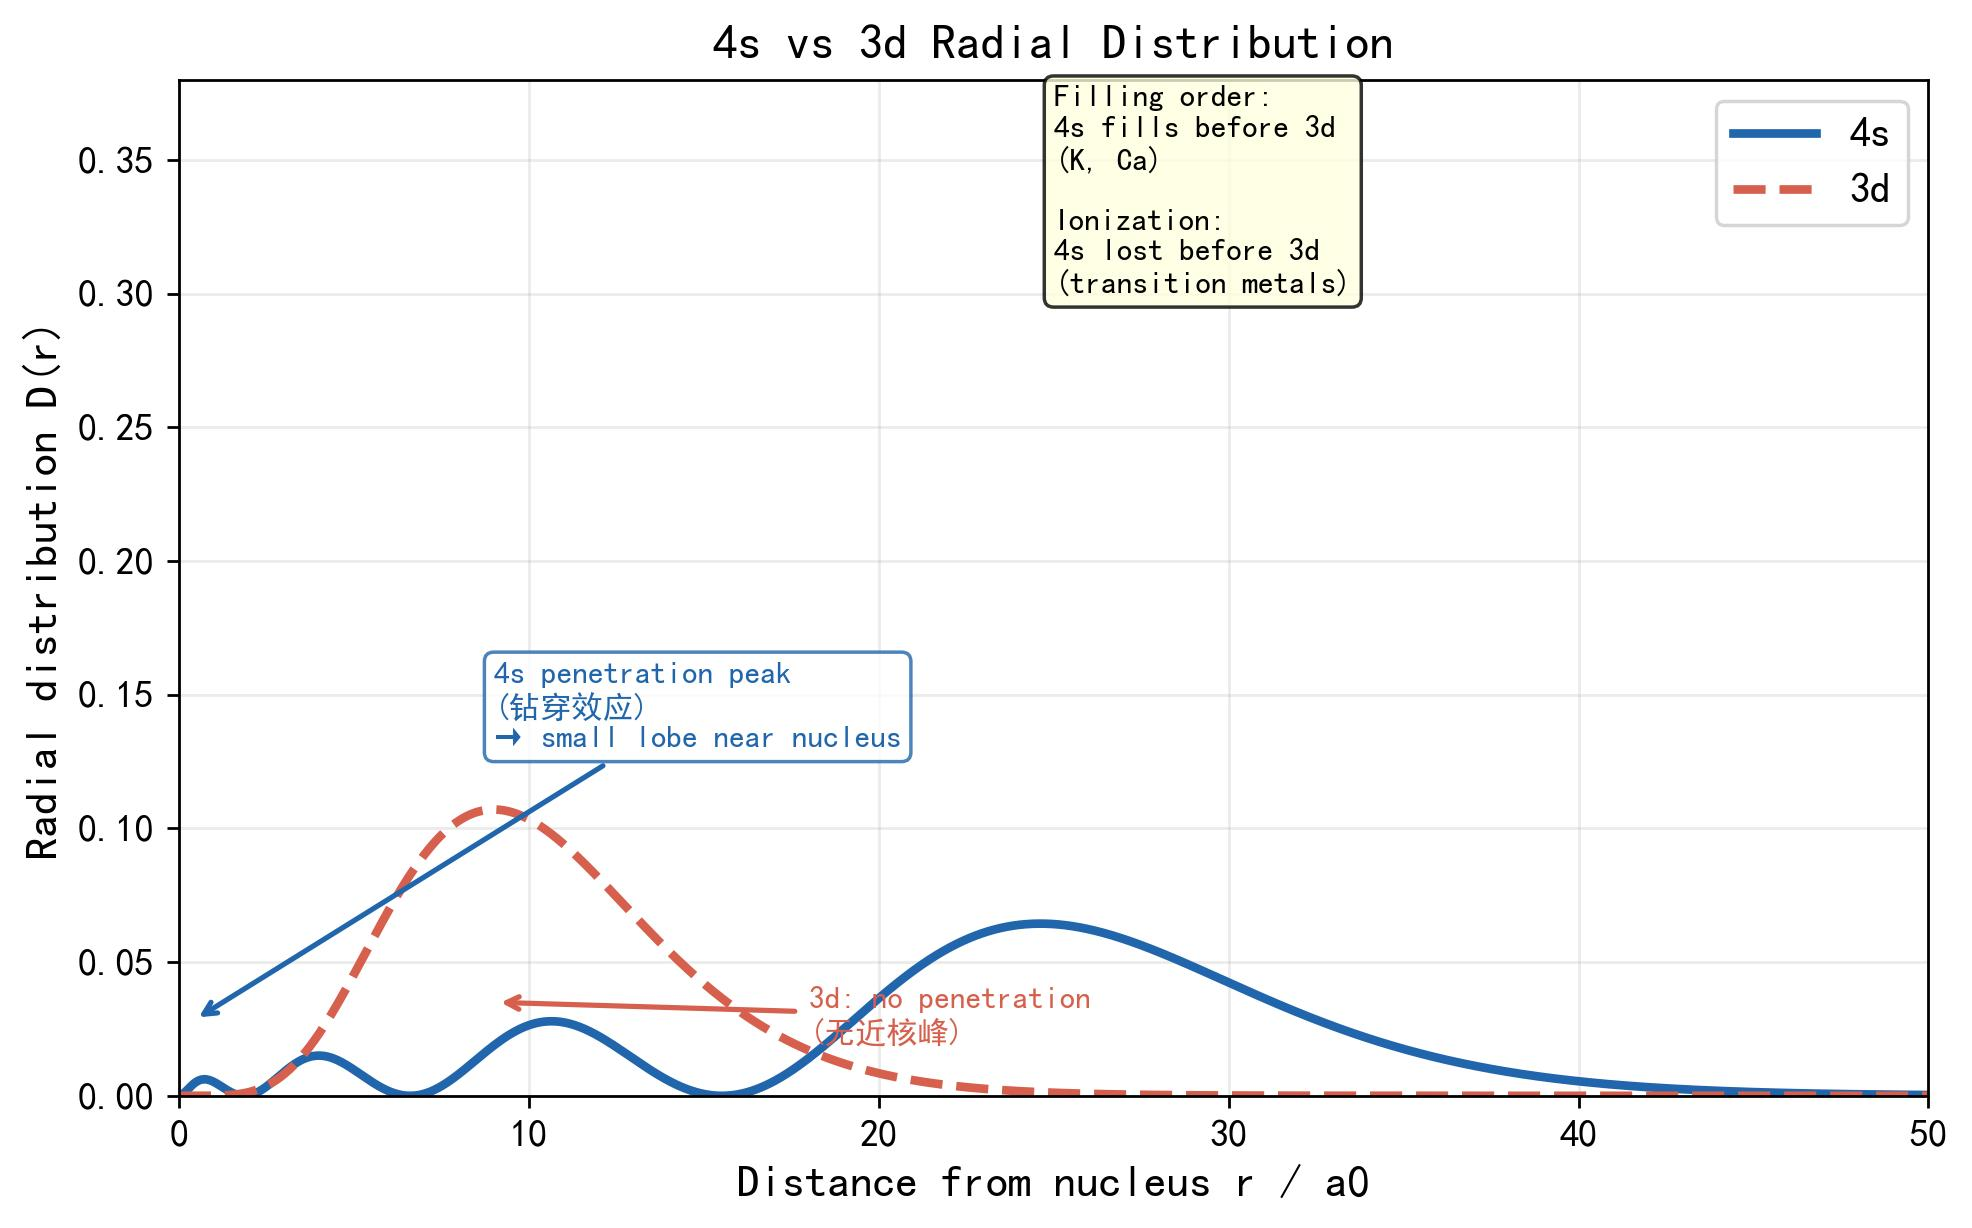
\includegraphics[width=0.45\textwidth,keepaspectratio]{media/11-22-4s-3d-radial-distribution.jpg}
\caption{图 4s与3d径向分布对比——4s在主峰外有靠近核的小峰（钻穿效应），3d无近核小峰。因此填充时4s先于3d（K、Ca），失电子时4s也先于3d。（普化原理第4版 图11.22）}
\end{figure}

\textbf{关键启示}：将角度分布图（11-13）与径向分布图对比可以看出，电子云的全貌需要\textbf{角度}和\textbf{径向}两个维度共同描述。

\begin{figure}[H]\centering
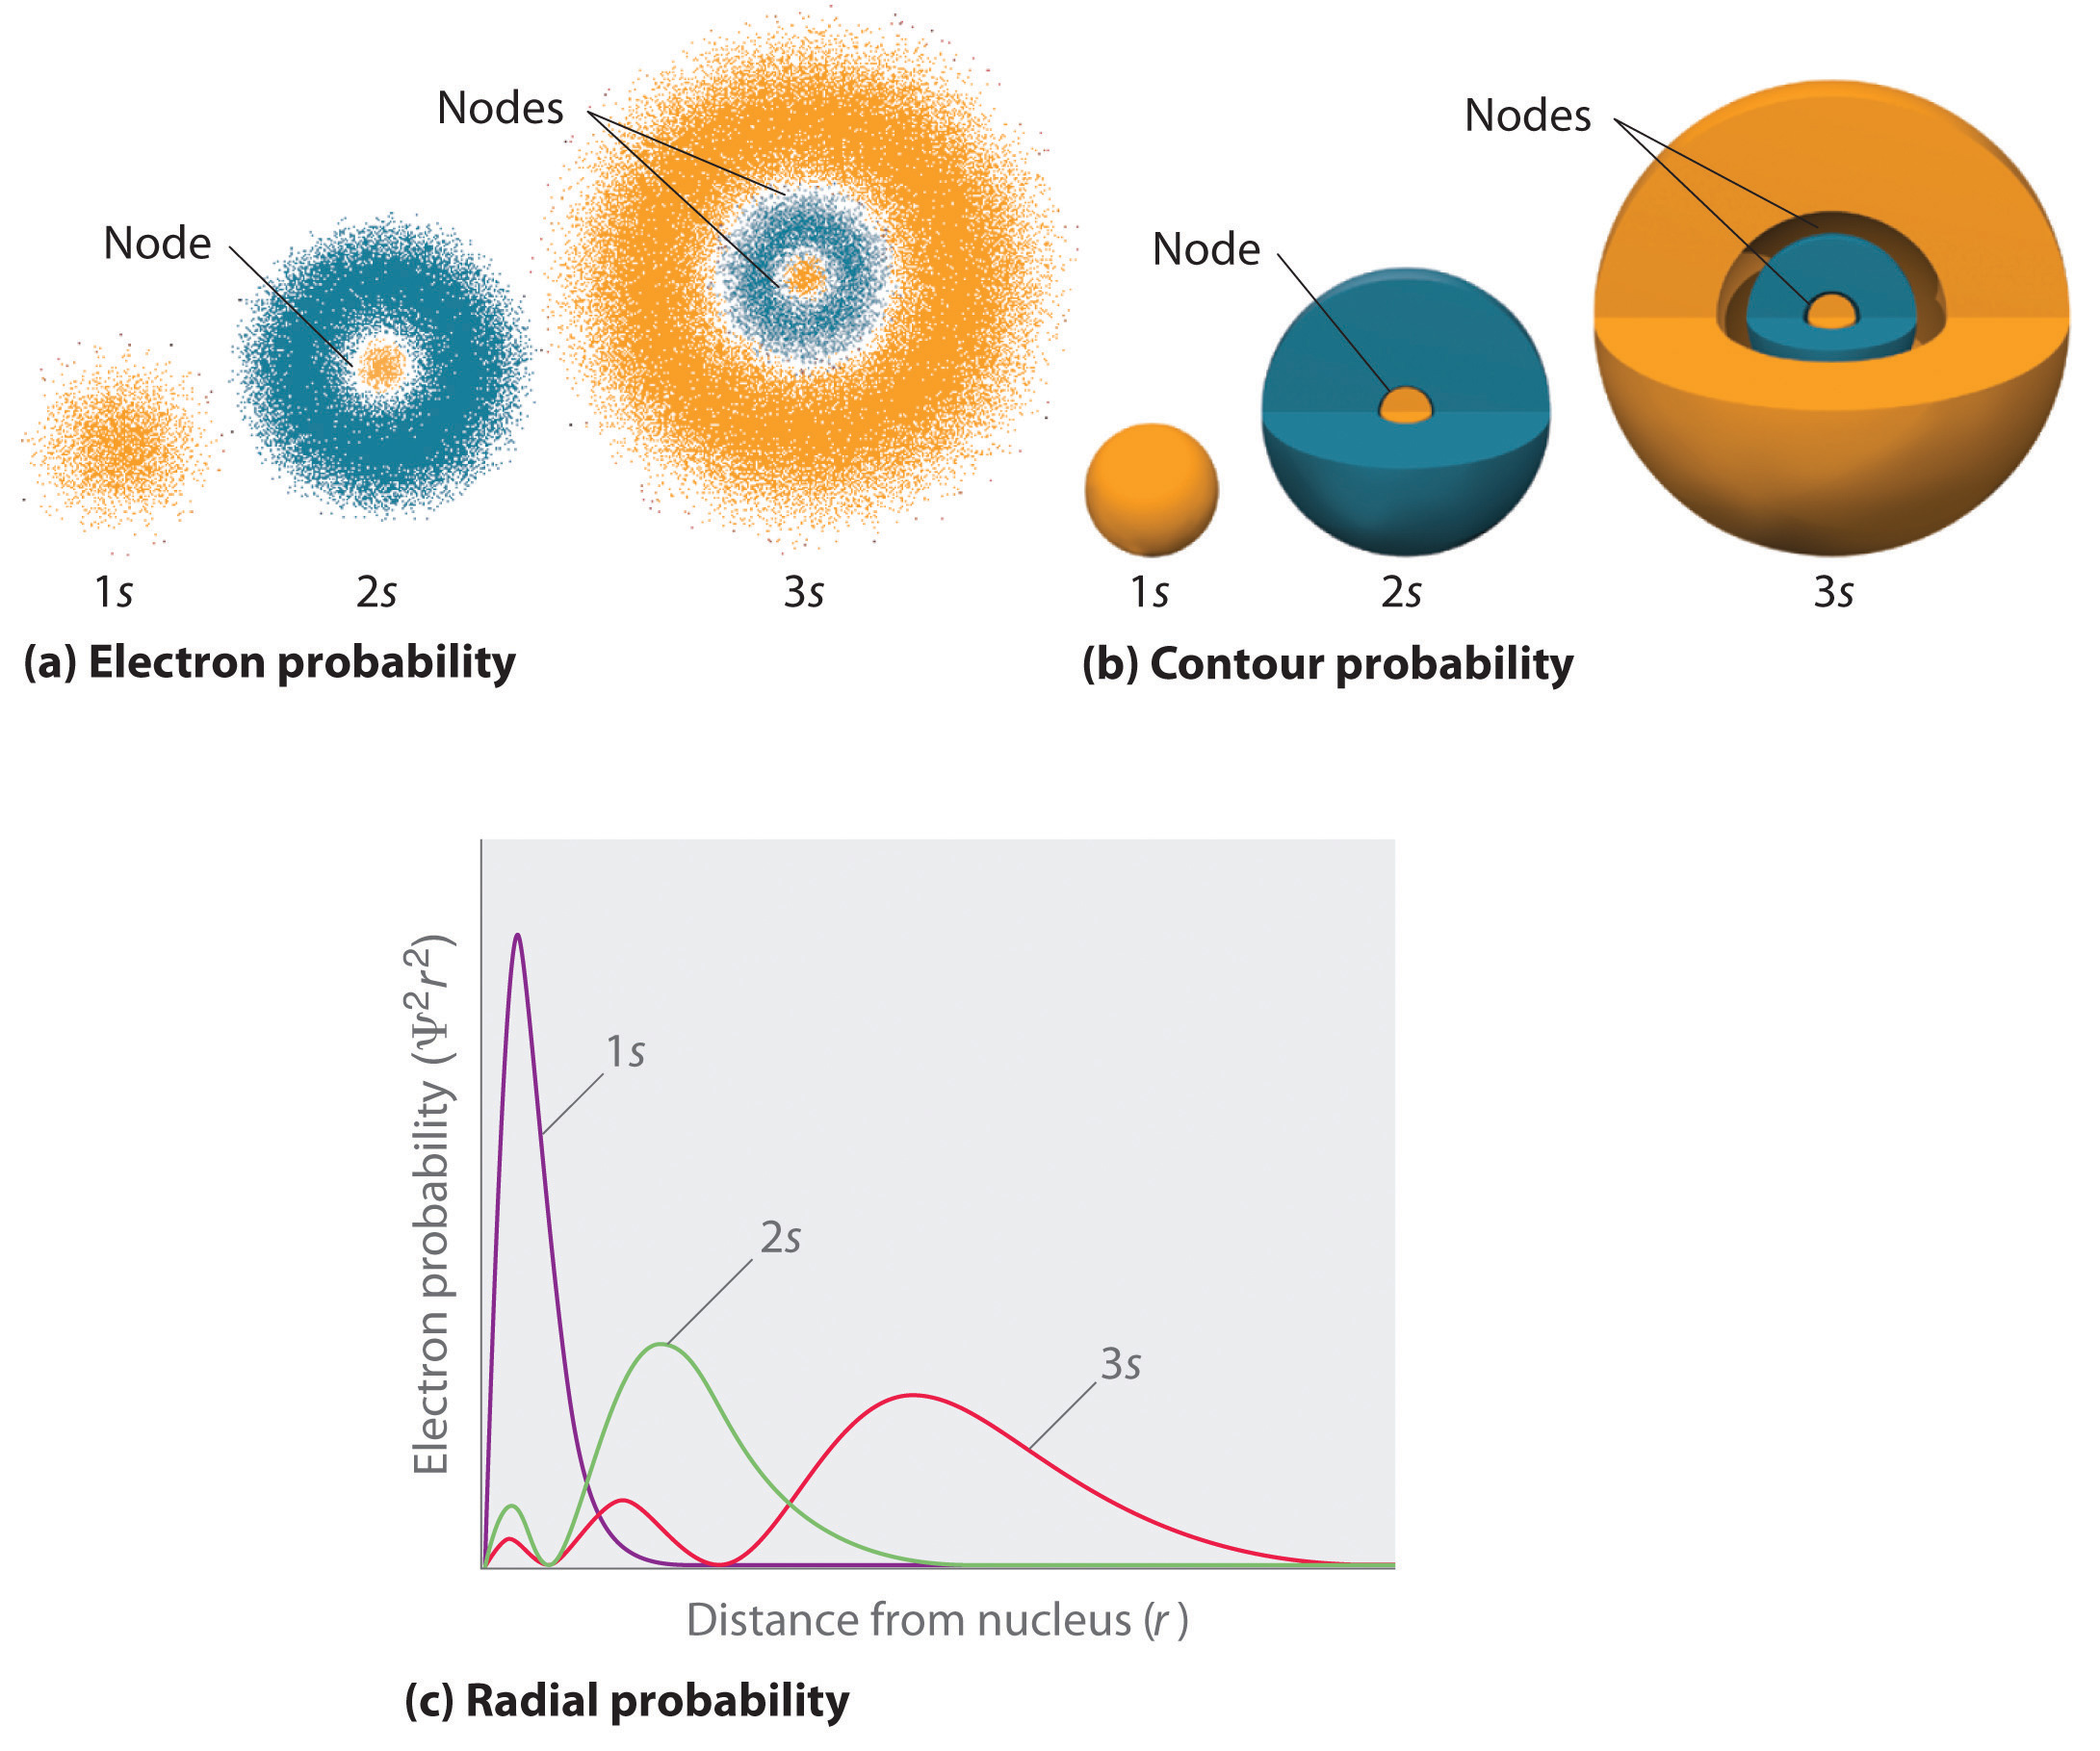
\includegraphics[width=0.45\textwidth,keepaspectratio]{media/orbital_density_1s_2s_3s.jpg}
\caption{图 s轨道径向概率密度分布——1s一个峰（最靠近核），2s两个峰，3s三个峰。最高峰位置随n增大而外移。近核小峰（钻穿）是s轨道能量低于同层p、d的原因。（普化原理第4版）}
\end{figure}

\paragraph{\texorpdfstring{（3）磁量子数 \(m_l\)------空间取向}{（3）磁量子数 m\_l------空间取向}}\label{ux78c1ux91cfux5b50ux6570-m_lux7a7aux95f4ux53d6ux5411}

\textbf{简并度}：

{\def\LTcaptype{none} % do not increment counter
\begin{longtable}[]{@{}
  >{\centering\arraybackslash}p{(\linewidth - 6\tabcolsep) * \real{0.2778}}
  >{\raggedright\arraybackslash}p{(\linewidth - 6\tabcolsep) * \real{0.2222}}
  >{\centering\arraybackslash}p{(\linewidth - 6\tabcolsep) * \real{0.2778}}
  >{\raggedright\arraybackslash}p{(\linewidth - 6\tabcolsep) * \real{0.2222}}@{}}
\toprule\noalign{}
\begin{minipage}[b]{\linewidth}\centering
\(l\)
\end{minipage} & \begin{minipage}[b]{\linewidth}\raggedright
\(m_l\) 取值
\end{minipage} & \begin{minipage}[b]{\linewidth}\centering
轨道数
\end{minipage} & \begin{minipage}[b]{\linewidth}\raggedright
轨道名称
\end{minipage} \\
\midrule\noalign{}
\endhead
\bottomrule\noalign{}
\endlastfoot
0 (s) & \(m_l=0\) & \textbf{1} & s \\
1 (p) & \(m_l=-1,0,+1\) & \textbf{3} & \(p_x, p_y, p_z\) \\
2 (d) & \(m_l=-2,-1,0,+1,+2\) & \textbf{5} & \(d_{xy}, d_{xz}, d_{yz}, d_{x^2-y^2}, d_{z^2}\) \\
3 (f) & \(m_l=-3,-2,-1,0,+1,+2,+3\) & \textbf{7} & f 七种取向 \\
\end{longtable}
}

\paragraph{\texorpdfstring{（4）自旋量子数 \(m_s\)------电子自旋}{（4）自旋量子数 m\_s------电子自旋}}\label{ux81eaux65cbux91cfux5b50ux6570-m_sux7535ux5b50ux81eaux65cb}

\begin{itemize}
\tightlist
\item
  取值：\(+\frac{1}{2}\)（↑）或 \(-\frac{1}{2}\)（↓）
\end{itemize}

\paragraph{（5）轨道数与电子容量综合表}\label{ux8f68ux9053ux6570ux4e0eux7535ux5b50ux5bb9ux91cfux7efcux5408ux8868}

{\def\LTcaptype{none} % do not increment counter
\begin{longtable}[]{@{}clccc@{}}
\toprule\noalign{}
\(n\) (能层) & \(l\) (亚层) & 轨道数 & 亚层最大电子数 & 该层总电子数 \\
\midrule\noalign{}
\endhead
\bottomrule\noalign{}
\endlastfoot
1 & 1s (0) & 1 & 2 & 2 \\
2 & 2s (0), 2p (1) & 1+3=4 & 2+6=8 & 8 \\
3 & 3s (0), 3p (1), 3d (2) & 1+3+5=9 & 2+6+10=18 & 18 \\
4 & 4s (0), 4p (1), 4d (2), 4f (3) & 1+3+5+7=16 & 2+6+10+14=32 & 32 \\
\end{longtable}
}

\begin{quote}
\textbf{⚠️ 易错点}：三个量子数 \((n,l,\)m\_l\()\) 确定一个\textbf{原子轨道}，四个量子数 \((n,l,\)m\_l\(,m_s)\) 确定一个\textbf{电子状态}。Pauli不相容原理：同一原子中无四个量子数完全相同的两个电子 ⇔ 每个轨道最多2个自旋相反的电子。
\end{quote}

------

\subsubsection{2.3 氢原子与多电子原子的能级}\label{ux6c22ux539fux5b50ux4e0eux591aux7535ux5b50ux539fux5b50ux7684ux80fdux7ea7}

\paragraph{① 氢原子（单电子体系）}\label{ux6c22ux539fux5b50ux5355ux7535ux5b50ux4f53ux7cfb}

\[E_n = -13.6 \cdot \frac{1}{n^2}\ \mathrm{eV}\]

\(n\) 相同但 \(l\) 不同的轨道------如 \(3s\)、\(3p\)、\(3d\)------能量完全相同（简并）。

\paragraph{② 多电子原子：屏蔽效应}\label{ux591aux7535ux5b50ux539fux5b50ux5c4fux853dux6548ux5e94}

\textbf{屏蔽效应}：其他电子对核电荷的''遮挡''作用，使指定电子感受到的核电荷减小。

\[\boxed{Z^* = Z - \sigma}\]

\[E_i = -13.6 \cdot \frac{(Z^*)^2}{n^2}\ \mathrm{eV}\]

\paragraph{③ Slater规则与定量计算}\label{slaterux89c4ux5219ux4e0eux5b9aux91cfux8ba1ux7b97}

\textbf{为什么需要 Slater 规则？}------屏蔽效应告诉我们''外层电子受内层屏蔽，能量升高''，但这只是定性描述。要定量知道''升高了多少''，就需要一个可计算的模型。Slater（1930）提出的这套规则，就是用量子力学近似计算屏蔽常数的实用工具。

电子分组：\[(1s)(2s,2p)(3s,3p)(3d)(4s,4p)(4d)(4f)(5s,5p)\dots\]

\textbf{关键观察}：为什么 \((ns,np)\) 合为同组而 \((nd)\) 单独一组？因为 s 和 p 轨道在空间分布上有重叠（钻穿能力相近），且光谱数据表明它们对彼此的屏蔽行为一致；而 d 轨道的钻穿能力明显弱于 s 和 p，屏蔽行为完全不同。

\begin{figure}[H]\centering
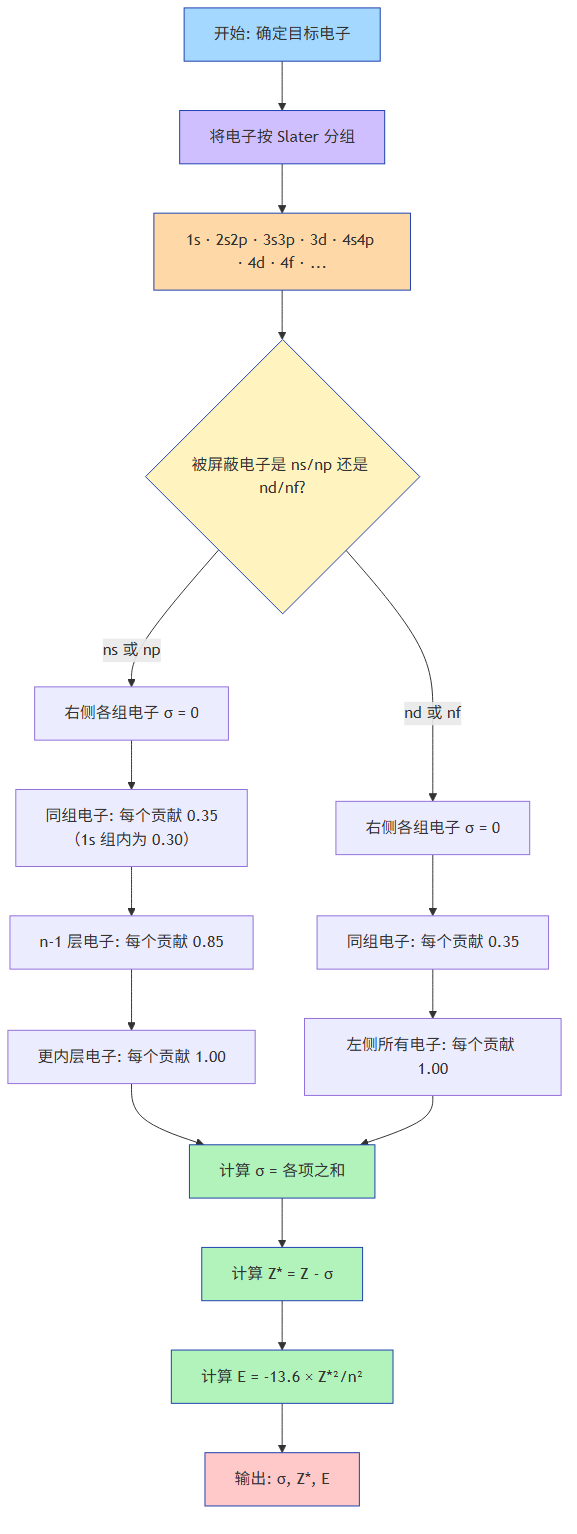
\includegraphics[width=0.45\textwidth,keepaspectratio]{media/excalidraw-原子结构-slater-rules-flowchart.png}
\caption{图 Slater规则计算流程图——从电子分组、确定被屏蔽电子、按四条规则逐组计算屏蔽常数σ，到计算有效核电荷Z}
\end{figure}

\textbf{口诀}：右不看，同0.35（1s 0.30）；ns/np：减一层0.85，再内全1.00；nd/nf：左边全都1.00。总和\(\sigma\)，\(Z^* = Z - \sigma\)，\(E = -13.6 (Z^*)^2/n^2\)。

\textbf{Slater规则四条}：

\begin{enumerate}
\def\labelenumi{\arabic{enumi}.}
\tightlist
\item
  \textbf{右侧忽略}：位于被屏蔽电子\textbf{右侧（更高n）} 的各组电子，屏蔽可忽略（\(\sigma = 0\)）
\item
  \textbf{同组屏蔽}：同组电子之间，每个贡献 \textbf{0.35}（但1s组内为 \textbf{0.30}------因为1s电子离核最近、电子云最紧密，彼此间的屏蔽效率略低于外层电子）
\item
  \textbf{相邻内组（ns/np）}：被屏蔽电子为 \(ns\) 或 \(np\) 时，\((n-1)\) 层电子贡献 \textbf{0.85}，更内层贡献 \textbf{1.00}
\item
  \textbf{相邻内组（nd/nf）}：被屏蔽电子为 \(nd\) 或 \(nf\) 时，其左侧\textbf{所有}电子贡献 \textbf{1.00}
\end{enumerate}

\textbf{Slater 规则的用途}：①\textbf{定量解释能级分裂和能级交错}------Cotton 图背后就是不同轨道 \(Z^*\) 的差异在随 Z 变化（见下方 Ti 示例）；②\textbf{估算 Allred-Rochow 电负性}（电负性 \(\propto Z^*/r^2\)）；③建立''屏蔽是可计算可验证''的量化认知，为后续 SCF 方法做铺垫。Slater 规则是近似方法，对 d/f 电子误差较大，更精确的 SCF 计算留待第三轮。

\textbf{示例1：Na原子（Z=11）} 分组：\((1s)^2(2s,2p)^8(3s)^1\)

{\def\LTcaptype{none} % do not increment counter
\begin{longtable}[]{@{}
  >{\raggedright\arraybackslash}p{(\linewidth - 6\tabcolsep) * \real{0.2353}}
  >{\raggedright\arraybackslash}p{(\linewidth - 6\tabcolsep) * \real{0.2353}}
  >{\raggedleft\arraybackslash}p{(\linewidth - 6\tabcolsep) * \real{0.2353}}
  >{\centering\arraybackslash}p{(\linewidth - 6\tabcolsep) * \real{0.2941}}@{}}
\toprule\noalign{}
\begin{minipage}[b]{\linewidth}\raggedright
电子
\end{minipage} & \begin{minipage}[b]{\linewidth}\raggedright
\(\sigma\) 计算
\end{minipage} & \begin{minipage}[b]{\linewidth}\raggedleft
\(Z^*\)
\end{minipage} & \begin{minipage}[b]{\linewidth}\centering
\(E = -13.6 \cdot (Z^*)^2/n^2\)
\end{minipage} \\
\midrule\noalign{}
\endhead
\bottomrule\noalign{}
\endlastfoot
1s & \(1 \times 0.30 = 0.30\) & 10.70 & \(-1557\ \mathrm{eV}\) \\
2s/2p & \(7 \times 0.35 + 2 \times 0.85 = 4.15\) & 6.85 & \(-160\ \mathrm{eV}\) \\
\textbf{3s} & \(8 \times 0.85 + 2 \times 1.00 = 8.80\) & \textbf{2.20} & \textbf{\(-7.3\ \mathrm{eV}\)} \\
\end{longtable}
}

\textbf{解读}：Na 的 3s 电子 \(Z^* = 2.20\)，远低于核电荷 +11------这就是为什么最外层电子能量如此之高（仅 -7.3 eV），化学性质活泼。如果完全没有屏蔽，3s 电子能量应为 \(-13.6 \times 11^2 / 9 = -183\ \mathrm{eV}\)------比实际值低 \textbf{25 倍}！屏蔽效应不是''微调''，而是数量级级别的修正。

\textbf{示例2：Ti原子（Z=22）} 分组：\((1s)^2(2s,2p)^8(3s,3p)^8(3d)^2(4s)^2\)

{\def\LTcaptype{none} % do not increment counter
\begin{longtable}[]{@{}
  >{\raggedright\arraybackslash}p{(\linewidth - 6\tabcolsep) * \real{0.2353}}
  >{\raggedright\arraybackslash}p{(\linewidth - 6\tabcolsep) * \real{0.2353}}
  >{\raggedleft\arraybackslash}p{(\linewidth - 6\tabcolsep) * \real{0.2353}}
  >{\centering\arraybackslash}p{(\linewidth - 6\tabcolsep) * \real{0.2941}}@{}}
\toprule\noalign{}
\begin{minipage}[b]{\linewidth}\raggedright
电子
\end{minipage} & \begin{minipage}[b]{\linewidth}\raggedright
\(\sigma\) 计算
\end{minipage} & \begin{minipage}[b]{\linewidth}\raggedleft
\(Z^*\)
\end{minipage} & \begin{minipage}[b]{\linewidth}\centering
\(E\)
\end{minipage} \\
\midrule\noalign{}
\endhead
\bottomrule\noalign{}
\endlastfoot
3p & \(7\times0.35 + 8\times0.85 + 2\times1.00 = 11.25\) & 10.75 & \(-174.6\ \mathrm{eV}\) \\
\textbf{3d} & \(1\times0.35 + 8\times1.00 + 8\times1.00 + 2\times1.00 = 18.35\) & \textbf{3.65} & \textbf{\(-20.1\ \mathrm{eV}\)} \\
\end{longtable}
}

\[\boxed{E_{3p} = -174.6\ \mathrm{eV} \ll E_{3d} = -20.1\ \mathrm{eV}}\]

\textbf{关键发现}：同 \(n=3\) 层，\(3p\) 和 \(3d\) 能量相差近 \textbf{9 倍}！这就是能级分裂的定量来源。\(3d\) 钻穿弱 → 内层对它屏蔽完全（\(\sigma_{3d}=18.35\)）→ \(Z^*\) 小 → 能量高。对照 Cotton 图中 \(E_{3d} > E_{3p}\) 的趋势，两者完全一致------\textbf{Slater 计算和 Cotton 图从定量、定性两个角度互相印证}。

------

\paragraph{③ 练习：Ti的3d电子屏蔽前后能量差}\label{ux7ec3ux4e60tiux76843dux7535ux5b50ux5c4fux853dux524dux540eux80fdux91cfux5dee}

假设完全没有屏蔽（\(\sigma = 0\)）：

\[E_{3d}(\text{无屏蔽}) = -13.6 \times \frac{22^2}{3^2} = -13.6 \times \frac{484}{9} = -731\ \mathrm{eV}\]

\[\Delta E = (-731) - (-20.1) = -711\ \mathrm{eV}\]

屏蔽使3d能量升高了711 eV！这个差值比许多化学键的键能（\textasciitilde200-400 kJ/mol ≈ 2-4 eV/原子）高出\textbf{两个数量级}------说明屏蔽效应是决定原子中电子能量的主导因素。

\paragraph{④ 钻穿效应------能级分裂的微观解释}\label{ux94bbux7a7fux6548ux5e94ux80fdux7ea7ux5206ux88c2ux7684ux5faeux89c2ux89e3ux91ca}

\textbf{钻穿效应}：外层电子钻入内层空间靠近原子核的现象。钻穿能力：\(ns > np > nd > nf\)

\begin{quote}
💡 \textbf{深层理解}：「3d 电子被 3s/3p 电子云遮挡------就像躲在盾牌后面感受不到核的引力一样。」
\end{quote}

📌 \textbf{理解要点}：``4s 和 3d 谁的能量低？直觉是 3d------n 小。但径向分布图显示：4s 的电子云有一个小峰钻到离核很近的地方------感受到的核电荷更大→能量更低。3d 没有这个小峰------被外面的电子云屏蔽了。''

\paragraph{⑤ 鲍林近似能级图与徐光宪规则}\label{ux9c8dux6797ux8fd1ux4f3cux80fdux7ea7ux56feux4e0eux5f90ux5149ux5baaux89c4ux5219}

美国化学家 Pauling 根据大量原子光谱实验数据，总结出多电子原子中各轨道能量的相对高低顺序------\textbf{鲍林近似能级图}。这不是理论推导的结果，而是实验归纳的产物：光谱中每一根谱线对应一个能级跃迁，Pauling 通过对数以千计谱线的系统分析，反推出了轨道的能量顺序。

\begin{verbatim}
第一能级组：1s
第二能级组：2s → 2p
第三能级组：3s → 3p
第四能级组：4s → 3d → 4p
第五能级组：5s → 4d → 5p
第六能级组：6s → 4f → 5d → 6p
第七能级组：7s → 5f → 6d → 7p
\end{verbatim}

\begin{figure}[H]\centering
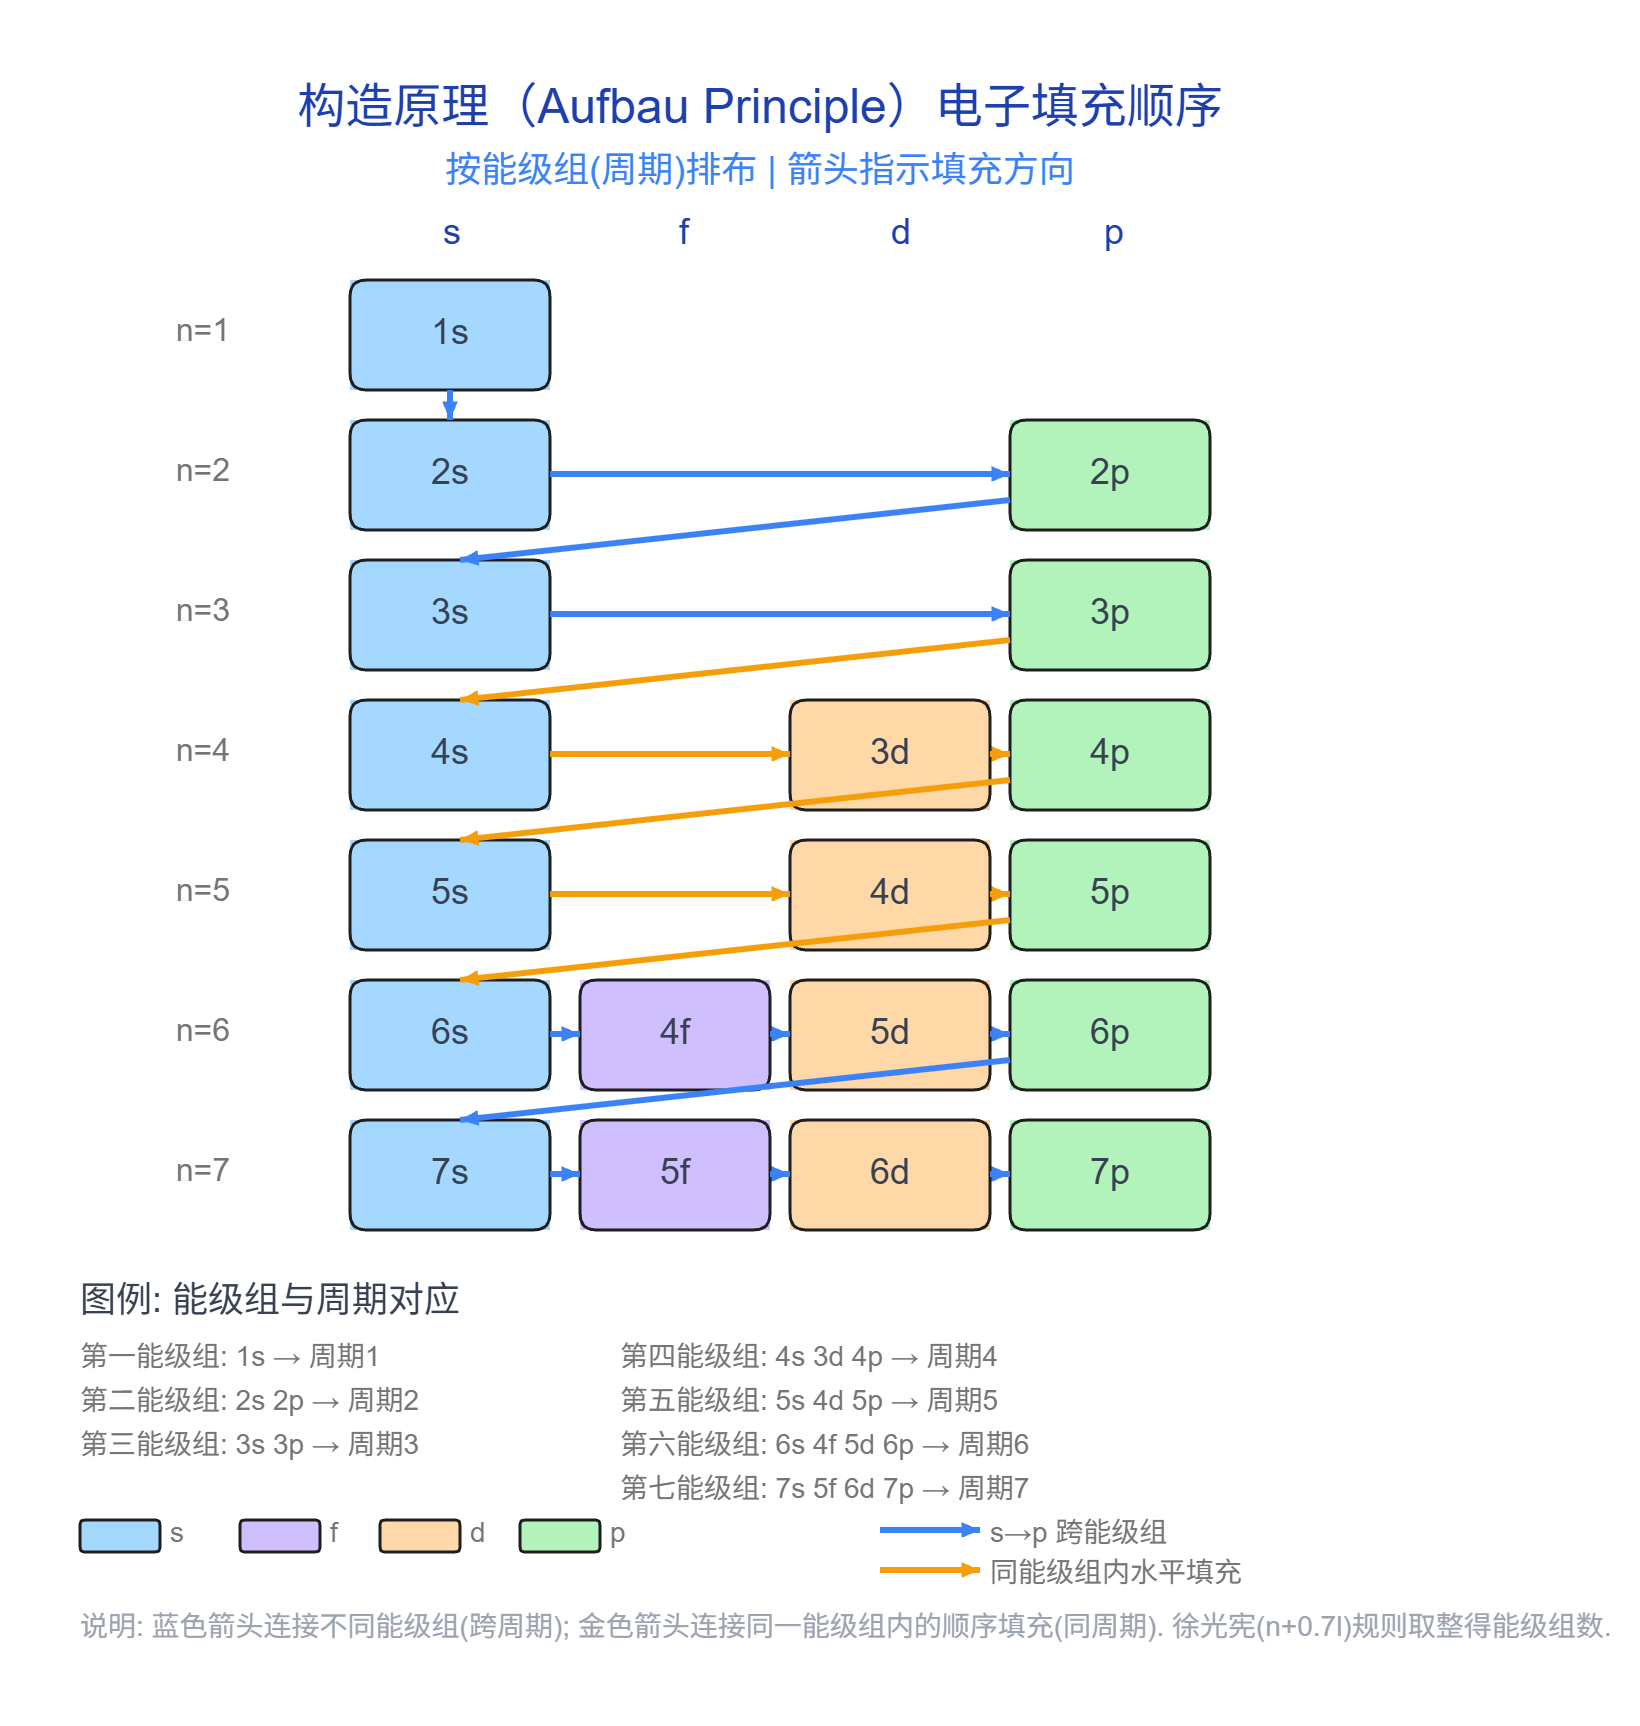
\includegraphics[width=0.5\textwidth,keepaspectratio]{media/构造原理-填充顺序.matrix.png}
\caption{图 构造原理电子填充顺序矩阵图——按轨道类型(s/f/d/p)与主量子数(n)排布，箭头指示填充路径。蓝色箭头为跨能级组(周期间)跳转，金色箭头为能级组内(同周期)水平填充。}
\end{figure}

\textbf{能级组与周期表的对应关系}：第 \(n\) 能级组对应周期 \(n\)------能级组的个数直接决定了元素周期表的行数。第一能级组（1s）→ 第一周期 2 种元素；第二+第三能级组（2s2p+3s3p）→ 第二、三周期各 8 种；第四能级组（4s3d4p）→ 第四周期 18 种。\textbf{能级组的容量 = 周期的宽度}。

\textbf{徐光宪（\(n+0.7l\)）规则}：将 Pauling 的图示经验总结为一个简洁的定量公式------\((n+0.7l)\) 值取整，即为该轨道所在的能级组数。

{\def\LTcaptype{none} % do not increment counter
\begin{longtable}[]{@{}lcc@{}}
\toprule\noalign{}
轨道 & \(n+0.7l\) & 能级组 \\
\midrule\noalign{}
\endhead
\bottomrule\noalign{}
\endlastfoot
4s & 4+0.7×0 = \textbf{4.0} & \textbf{4} \\
3d & 3+0.7×2 = \textbf{4.4} & \textbf{4} \\
4p & 4+0.7×1 = \textbf{4.7} & \textbf{4} \\
5s & 5+0.7×0 = \textbf{5.0} & \textbf{5} \\
4f & 4+0.7×3 = \textbf{6.1} & \textbf{6} \\
\end{longtable}
}

为什么是 0.7？这并非任意选取。\(0.7l\) 项本质上是对\textbf{钻穿效应}的定量补偿：\(l\) 越大 → 钻穿越弱 → 受屏蔽越多 → 有效能量越高 → 需要加一个正的修正项。s 电子（\(l=0\)）钻穿最强，修正为 0；p 电子（\(l=1\)）钻穿次之，修正 0.7；d 电子（\(l=2\)）钻穿更弱，修正 1.4------这就是为什么 3d 虽然 \(n\) 更小（\(n=3\)），却能级却位于 4s 之上（\(3+1.4=4.4>4.0\)），与第四周期而非第三周期对应。

\begin{figure}[H]\centering
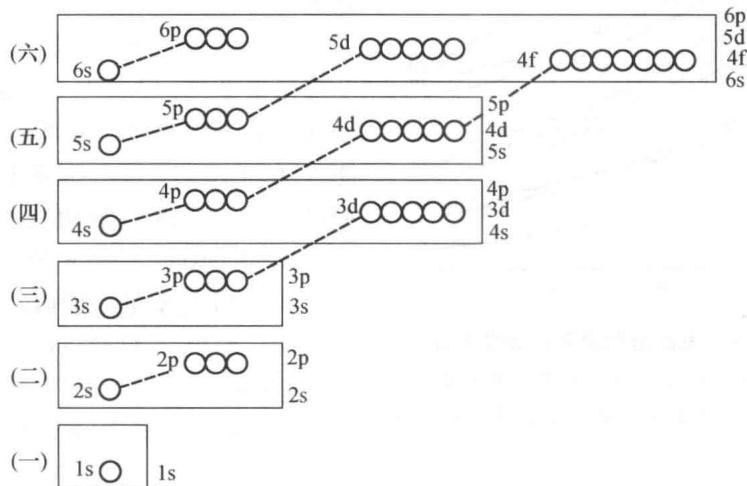
\includegraphics[width=0.45\textwidth,keepaspectratio]{media/11-19-pauling-energy-levels.jpg}
\caption{图 Pauling 近似能级图——按轨道能量由低到高排列，以水平线高低代表能量相对高低，每个方框代表一个轨道，箭头指示电子填入顺序。能级组以虚线方框标出（普化原理第4版 图11.19）}
\end{figure}

\begin{figure}[H]\centering
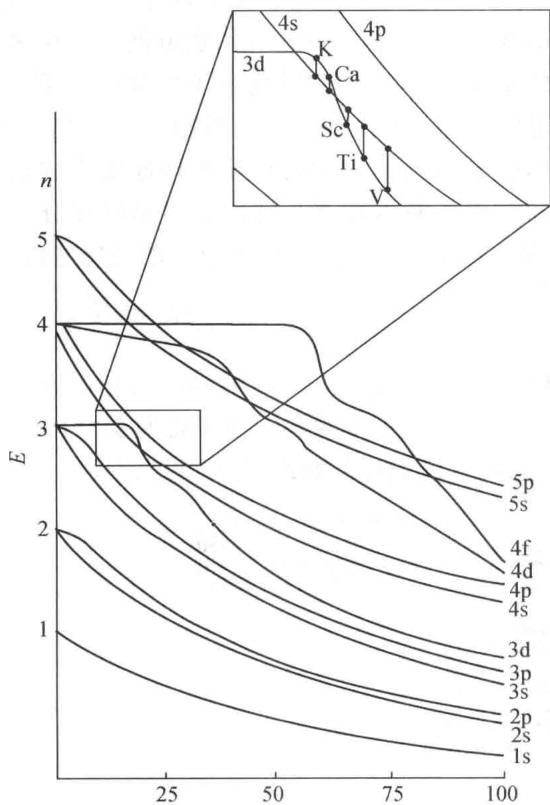
\includegraphics[width=0.45\textwidth,keepaspectratio]{media/11-20-cotton-orbital-energy-vs-Z.jpg}
\caption{图 多电子原子轨道能量随原子序数的变化（Cotton 能级图，F. A. Cotton, 1962）——横坐标为原子序数 Z，纵坐标为轨道能量 E。氢原子（Z=1）中同层轨道简并；随 Z 增大，核电荷增加使所有轨道能量单调下降，但 s 轨道（钻穿强、受屏蔽少）下降最快，p 轨道次之，d 轨道（钻穿弱、受屏蔽多）下降最慢。由此产生能级分裂和能级交错：K、Ca 处 E4s < E3d → 4s 先于 3d 填充；Z ≥ 21 后 E3d 降至 E4s 以下 → 失电子时先失 4s（普化原理第4版 图11.20 / Cotton, F. A.）}
\end{figure}

\begin{quote}
⚠️ \textbf{核心辨析}：Pauling 能级图描述的是\textbf{电子填充顺序}，Cotton 图展示的是\textbf{轨道实际能量随 Z 的动态变化}。二者不矛盾------填充顺序反映的是整个原子基态的总能量最低原则，而轨道实际能量受屏蔽和钻穿的共同调控，随 Z 连续变化。\textbf{填充顺序用 Pauling 图，理解能量本质看 Cotton 图。}
\end{quote}

------

\subsection{三、基态原子核外电子排布}\label{ux4e09ux57faux6001ux539fux5b50ux6838ux5916ux7535ux5b50ux6392ux5e03}

\textbf{关联知识点}：电子排布 · 元素周期律 · 电离能 · 电负性

\subsubsection{3.1 电子排布三原则}\label{ux7535ux5b50ux6392ux5e03ux4e09ux539fux5219}

\textbf{口诀}：电子填入先低能，能级组内按顺序：\(1s \to 2s \to 2p \to 3s \to 3p \to 4s \to 3d \to 4p \to 5s \to 4d \to 5p \to 6s \to 4f \to 5d \to 6p \to \dots\)

\paragraph{（1）构造原理（Aufbau Principle）}\label{ux6784ux9020ux539fux7406aufbau-principle}

\textbf{Aufbau} 在德语中意为''构建''（building up）------从氢原子开始，每增加一个质子（核电荷 +1）就增加一个电子，电子按轨道能量由低到高依次填入。对初学者而言，这条规则最直接、最容易使用，但\textbf{它只是经验总结，不是物理定律}------后面会看到，Cr 和 Cu 并不严格遵循这一顺序。

填充顺序遵循 Pauling 近似能级图（§2.3⑤）：

\[1s \to 2s \to 2p \to 3s \to 3p \to 4s \to 3d \to 4p \to 5s \to 4d \to 5p \to 6s \to 4f \to 5d \to 6p \to \dots\]

\paragraph{（2）Pauli不相容原理}\label{pauliux4e0dux76f8ux5bb9ux539fux7406}

\textbf{正式表述}：同一原子中，不可能有四个量子数 \((n,l,m_l,m_s)\) 完全相同的两个电子。

\textbf{等价表述}：每个原子轨道最多容纳 2 个自旋相反的电子。

\begin{figure}[H]\centering
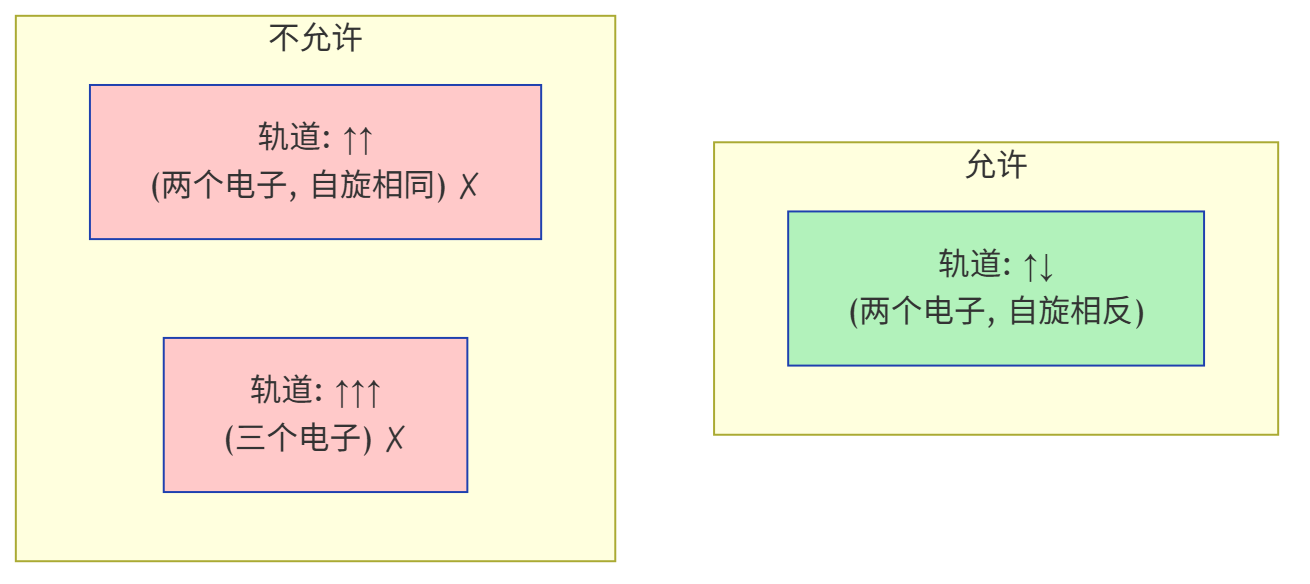
\includegraphics[width=0.45\textwidth,keepaspectratio]{media/excalidraw-原子结构-电子排布三原则-2.png}
\caption{图 Pauli不相容原理示意图——同一原子轨道最多容纳2个自旋相反的电子，四个量子数(n,l,m_l,m_s)完全相同的两个电子不允许存在}
\end{figure}

\textbf{物理背景}：Pauli 原理是量子力学中的一条基本定理，源于电子作为\textbf{费米子}的本性------两个全同费米子不能占据相同的量子态。它不是''经验规则''，而是\textbf{基本物理定律}。有了这条原理，元素周期表的结构才得以解释：\(n=1\) 层最多 2 个元素（H, He），\(n=2\) 层最多 8 个（Li→Ne），\(n=3\) 层最多 18 个------每一层''满了''就出现一个稀有气体，下一周期从头开始。

\textbf{范例}：Ca 的两个 4s 电子的量子数------电子1：\((n=4,l=0,\)m\_l\(=0,m_s=+1/2)\)；电子2：\((n=4,l=0,\)m\_l\(=0,m_s=-1/2)\)。前三个量子数完全相同，但自旋相反，符合 Pauli 原理。

\begin{quote}
⚠️ \textbf{常见误区}：\(m_s=0\) 不允许！\(m_s\) 必须为 \(+1/2\) 或 \(-1/2\)。写 \(m_s=0\) 的同学往往混淆了磁量子数 \(m_l=0\) 和自旋量子数 \(m_s=±1/2\)。
\end{quote}

\paragraph{（3）Hund规则}\label{hundux89c4ux5219}

\textbf{基本表述}：电子在简并轨道（能量相同，即 \(n,l\) 相同）上分布时，优先以自旋相同的方向分占不同轨道。

\textbf{物理来源}：Hund 规则的本质是\textbf{交换能}（exchange energy）驱动------当两个电子平行自旋占据不同轨道时，它们的波函数在空间上重合更少，库仑排斥小于反平行自旋的配对电子。这个能量差不大（通常 \textasciitilde1-2 eV），但足以决定基态排布。

\textbf{特例：半满/全满额外稳定性}------简并轨道处于\textbf{半充满}（\(\mathrm{p^3, d^5, f^7}\)）或\textbf{全充满}（\(\mathrm{p^6, d^{10}, f^{14}}\)）时，平行自旋数最大，交换能最大，体系能量特别低。

🔑 \textbf{深层逻辑}：Hund 规则不是''三条独立原则''之一------它是交换能的直接结果。理解这一点后，Cr 和 Cu 的特例就不再是''要背的例外''，而是''总能量最低原则的自然推论''。

\begin{quote}
💡 \textbf{易错提醒}：最高频错误------「Cr 不是 {[}Ar{]}4s\textsuperscript{2}3d\textsuperscript{4}------是 4s\textsuperscript{1}3d\textsuperscript{5}！」约有40\%的同学第一次都会写错。注意区分半满特例和一般情况。
\end{quote}

📌 \textbf{理解要点}：``Cr 不是 {[}Ar{]}4s\textsuperscript{2}3d\textsuperscript{4}------是 4s\textsuperscript{1}3d\textsuperscript{5}。Cu 不是 4s\textsuperscript{2}3d\textsuperscript{9}------是 4s\textsuperscript{1}3d\textsuperscript{10}。半满和全满稳定------但不要推广到所有过渡金属。只有 Cr 族和 Cu 族有这种特例。''

\subsubsection{3.2 电子排布的表示方法}\label{ux7535ux5b50ux6392ux5e03ux7684ux8868ux793aux65b9ux6cd5}

以N（Z=7）为例：\(1\mathrm{s}^2 2\mathrm{s}^2 2\mathrm{p}^3\)（排布式），\([\mathrm{He}] 2\mathrm{s}^2 2\mathrm{p}^3\)（稀有气体简式），\(2\mathrm{s}^2 2\mathrm{p}^3\)（价电子构型）。

\subsubsection{3.3 常见元素基态电子排布}\label{ux5e38ux89c1ux5143ux7d20ux57faux6001ux7535ux5b50ux6392ux5e03}

\paragraph{主族元素（Z≤20）}\label{ux4e3bux65cfux5143ux7d20z20}

{\def\LTcaptype{none} % do not increment counter
\begin{longtable}[]{@{}lcllc@{}}
\toprule\noalign{}
元素 & Z & 电子排布式 & 价电子构型 & 未成对电子数 \\
\midrule\noalign{}
\endhead
\bottomrule\noalign{}
\endlastfoot
H & 1 & \textbf{1s\textsuperscript{1}} & 1s\textsuperscript{1} & 1 \\
He & 2 & \textbf{1s\textsuperscript{2}} & \textbf{1s\textsuperscript{2}} & 0 \\
Li & 3 & \textbf{{[}He{]}2s\textsuperscript{1}} & \textbf{2s\textsuperscript{1}} & \textbf{1} \\
Be & 4 & \textbf{{[}He{]}2s\textsuperscript{2}} & \textbf{2s\textsuperscript{2}} & \textbf{0} \\
B & 5 & \textbf{{[}He{]}2s\textsuperscript{2}2p\textsuperscript{1}} & \textbf{2s\textsuperscript{2}2p\textsuperscript{1}} & \textbf{1} \\
C & 6 & \textbf{{[}He{]}2s\textsuperscript{2}2p\textsuperscript{2}} & \textbf{2s\textsuperscript{2}2p\textsuperscript{2}} & \textbf{2} \\
N & 7 & \textbf{{[}He{]}2s\textsuperscript{2}2p\textsuperscript{3}} & \textbf{2s\textsuperscript{2}2p\textsuperscript{3}} & \textbf{3} \\
O & 8 & \textbf{{[}He{]}2s\textsuperscript{2}2p\textsuperscript{4}} & \textbf{2s\textsuperscript{2}2p\textsuperscript{4}} & \textbf{2} \\
F & 9 & \textbf{{[}He{]}2s\textsuperscript{2}2p\textsuperscript{5}} & \textbf{2s\textsuperscript{2}2p\textsuperscript{5}} & \textbf{1} \\
Ne & 10 & \textbf{{[}He{]}2s\textsuperscript{2}2p\textsuperscript{6}} & \textbf{2s\textsuperscript{2}2p\textsuperscript{6}} & 0 \\
Na & 11 & \textbf{{[}Ne{]}3s\textsuperscript{1}} & \textbf{3s\textsuperscript{1}} & 1 \\
Mg & 12 & \textbf{{[}Ne{]}3s\textsuperscript{2}} & \textbf{3s\textsuperscript{2}} & 0 \\
Al & 13 & \textbf{{[}Ne{]}3s\textsuperscript{2}3p\textsuperscript{1}} & \textbf{3s\textsuperscript{2}3p\textsuperscript{1}} & \textbf{1} \\
Si & 14 & \textbf{{[}Ne{]}3s\textsuperscript{2}3p\textsuperscript{2}} & \textbf{3s\textsuperscript{2}3p\textsuperscript{2}} & \textbf{2} \\
P & 15 & \textbf{{[}Ne{]}3s\textsuperscript{2}3p\textsuperscript{3}} & \textbf{3s\textsuperscript{2}3p\textsuperscript{3}} & \textbf{3} \\
S & 16 & \textbf{{[}Ne{]}3s\textsuperscript{2}3p\textsuperscript{4}} & \textbf{3s\textsuperscript{2}3p\textsuperscript{4}} & \textbf{2} \\
Cl & 17 & \textbf{{[}Ne{]}3s\textsuperscript{2}3p\textsuperscript{5}} & \textbf{3s\textsuperscript{2}3p\textsuperscript{5}} & \textbf{1} \\
Ar & 18 & \textbf{{[}Ne{]}3s\textsuperscript{2}3p\textsuperscript{6}} & \textbf{3s\textsuperscript{2}3p\textsuperscript{6}} & 0 \\
K & 19 & \textbf{{[}Ar{]}4s\textsuperscript{1}} & \textbf{4s\textsuperscript{1}} & 1 \\
Ca & 20 & \textbf{{[}Ar{]}4s\textsuperscript{2}} & \textbf{4s\textsuperscript{2}} & 0 \\
\end{longtable}
}

\paragraph{过渡元素（Z=21-30）}\label{ux8fc7ux6e21ux5143ux7d20z21-30}

{\def\LTcaptype{none} % do not increment counter
\begin{longtable}[]{@{}ccllr@{}}
\toprule\noalign{}
Z & 符号 & 名称 & 价电子排布 & 未成对电子数 \\
\midrule\noalign{}
\endhead
\bottomrule\noalign{}
\endlastfoot
21 & \textbf{Sc} & \textbf{钪} & \textbf{3d\textsuperscript{1}4s\textsuperscript{2}} & 1 \\
22 & \textbf{Ti} & \textbf{钛} & \textbf{3d\textsuperscript{2}4s\textsuperscript{2}} & 2 \\
23 & \textbf{V} & \textbf{钒} & \textbf{3d\textsuperscript{3}4s\textsuperscript{2}} & 3 \\
24 & \textbf{Cr} & \textbf{铬} & \textbf{3d\textsuperscript{5}4s\textsuperscript{1}} & \textbf{6} \\
25 & \textbf{Mn} & \textbf{锰} & \textbf{3d\textsuperscript{5}4s\textsuperscript{2}} & 5 \\
26 & \textbf{Fe} & \textbf{铁} & \textbf{3d\textsuperscript{6}4s\textsuperscript{2}} & 4 \\
27 & \textbf{Co} & \textbf{钴} & \textbf{3d\textsuperscript{7}4s\textsuperscript{2}} & 3 \\
28 & \textbf{Ni} & \textbf{镍} & \textbf{3d\textsuperscript{8}4s\textsuperscript{2}} & 2 \\
29 & \textbf{Cu} & \textbf{铜} & \textbf{3d\textsuperscript{10}4s\textsuperscript{1}} & \textbf{1} \\
30 & \textbf{Zn} & \textbf{锌} & \textbf{3d\textsuperscript{10}4s\textsuperscript{2}} & 0 \\
\end{longtable}
}

\textbf{主族元素（Z=31-36）}：Ga {[}Ar{]}3d\textsuperscript{10}4s\textsuperscript{2}4p\textsuperscript{1}、Ge 3d\textsuperscript{10}4s\textsuperscript{2}4p\textsuperscript{2}、As 3d\textsuperscript{10}4s\textsuperscript{2}4p\textsuperscript{3}、Se 3d\textsuperscript{10}4s\textsuperscript{2}4p\textsuperscript{4}、Br 3d\textsuperscript{10}4s\textsuperscript{2}4p\textsuperscript{5}、Kr 3d\textsuperscript{10}4s\textsuperscript{2}4p\textsuperscript{6}

\paragraph{第五周期过渡金属（Z=39-48）}\label{ux7b2cux4e94ux5468ux671fux8fc7ux6e21ux91d1ux5c5ez39-48}

{\def\LTcaptype{none} % do not increment counter
\begin{longtable}[]{@{}ccllrl@{}}
\toprule\noalign{}
Z & 符号 & 名称 & 价电子排布 & 未成对 & 特例 \\
\midrule\noalign{}
\endhead
\bottomrule\noalign{}
\endlastfoot
42 & \textbf{Mo} & 钼 & \textbf{4d\textsuperscript{5}5s\textsuperscript{1}} & 6 & 半满（同Cr） \\
43 & Tc & 锝 & 4d\textsuperscript{5}5s\textsuperscript{2} & 5 & \textbf{反例}------半满但保留5s\textsuperscript{2} \\
46 & \textbf{Pd} & 钯 & \textbf{4d\textsuperscript{10}} & 0 & 全满，5s全空 \\
47 & \textbf{Ag} & 银 & \textbf{4d\textsuperscript{10}5s\textsuperscript{1}} & 1 & 全满（同Cu） \\
\end{longtable}
}

\begin{quote}
\textbf{⚠️ 竞赛高频考点}：Pd的 \(4d^{10}\) 排布是唯一 \(5s\) 全空的钯系元素。4d系列特例比3d更复杂。
\end{quote}

\begin{quote}
💡 \textbf{易错提醒}：「填充 4s 先于 3d，失电子 4s 先于 3d」------入住顺序≠退房顺序，大约25\%的同学会混淆。类比：4s 像酒店大堂------入住时先到大堂（先填 4s），退房时也从大堂走（先失 4s）。
\end{quote}

\subsubsection{3.4 电子排布特例：半满/全满稳定化}\label{ux7535ux5b50ux6392ux5e03ux7279ux4f8bux534aux6ee1ux5168ux6ee1ux7a33ux5b9aux5316}

{\def\LTcaptype{none} % do not increment counter
\begin{longtable}[]{@{}
  >{\raggedright\arraybackslash}p{(\linewidth - 6\tabcolsep) * \real{0.2500}}
  >{\raggedright\arraybackslash}p{(\linewidth - 6\tabcolsep) * \real{0.2500}}
  >{\raggedright\arraybackslash}p{(\linewidth - 6\tabcolsep) * \real{0.2500}}
  >{\raggedright\arraybackslash}p{(\linewidth - 6\tabcolsep) * \real{0.2500}}@{}}
\toprule\noalign{}
\begin{minipage}[b]{\linewidth}\raggedright
元素
\end{minipage} & \begin{minipage}[b]{\linewidth}\raggedright
预期排布（机械套用构造原理）
\end{minipage} & \begin{minipage}[b]{\linewidth}\raggedright
实际排布
\end{minipage} & \begin{minipage}[b]{\linewidth}\raggedright
原因
\end{minipage} \\
\midrule\noalign{}
\endhead
\bottomrule\noalign{}
\endlastfoot
\textbf{Cr} (Z=24) & {[}Ar{]} 3d\textsuperscript{4}4s\textsuperscript{2} & {[}Ar{]} \textbf{3d\textsuperscript{5}4s\textsuperscript{1}} & 3d半满（d\textsuperscript{5}）额外稳定 \\
\textbf{Cu} (Z=29) & {[}Ar{]} 3d\textsuperscript{9}4s\textsuperscript{2} & {[}Ar{]} \textbf{3d\textsuperscript{10}4s\textsuperscript{1}} & 3d全满（d\textsuperscript{10}）额外稳定 \\
\end{longtable}
}

\textbf{竞赛扩展}：Mo(4d\textsuperscript{5}5s\textsuperscript{1})、Ag(4d\textsuperscript{10}5s\textsuperscript{1})、Pd(4d\textsuperscript{10})、Au(4f\textsuperscript{14}5d\textsuperscript{10}6s\textsuperscript{1})

\paragraph{统一解释：成对能 vs 轨道能级差（Rich 模型）}\label{ux7edfux4e00ux89e3ux91caux6210ux5bf9ux80fd-vs-ux8f68ux9053ux80fdux7ea7ux5deerich-ux6a21ux578b}

Cotton 图展示了轨道能量随 Z 的变化，但这只解释了''为什么填充顺序先 4s 后 3d''。要解释 Cr/Cu 以及更复杂的 Nb/Ru/Rh/Pd 反常，需要引入\textbf{成对能}（pairing energy，\(P\)）的概念：

\textbf{成对能}：当两个电子被迫进入同一轨道时，因库仑排斥而升高的能量。

Rich（1965）在 Cotton 图的基础上叠入成对能，提出一个统一模型：
- 3d 和 4s 轨道能量均随 Z 增大而下降，两条能级线之间夹着一个\textbf{成对能区间}
- 电子总是选择使总能量最低的排布------当轨道能级差 \textless{} 成对能时，``分散填''更有利（Cr 的 3d\textsuperscript{5}4s\textsuperscript{1}）；当轨道能级差 \textgreater{} 成对能时，``集中填''更有利（Cu 的 3d\textsuperscript{10}4s\textsuperscript{1}）

这个模型可以统一解释整个 d 区反常：
- \textbf{Cr}（Z=24）：4s 能量已低于''3d + 成对能'' → 分散填 3d\textsuperscript{5}4s\textsuperscript{1}
- \textbf{Cu}（Z=29）：3d 能量已低于''4s + 成对能'' → 集中填 3d\textsuperscript{10}4s\textsuperscript{1}
- \textbf{Nb}（Z=41, 4d\textsuperscript{4}5s\textsuperscript{1}）、\textbf{Ru}（Z=44, 4d\textsuperscript{7}5s\textsuperscript{1}）、\textbf{Rh}（Z=45, 4d\textsuperscript{8}5s\textsuperscript{1}）--- 4d 系列成对能更大，反常更多
- \textbf{Pd}（Z=46, 4d\textsuperscript{10}）：成对能驱动 → 5s 全空，4d 全满

\textbf{一句话总结}：半满/全满是结果，不是原因。真正的驱动力是\textbf{成对能与轨道能级差的竞争}。

\begin{quote}
🧪 \textbf{兴趣阅读：Sc 的 Koopmans 能量分解------``先填 4s''是一道可计算的物理题}
上面的解释用 Rich 图定性说明了成对能与轨道能级差的竞争。但你知道吗------"先填 4s 又先电离 4s" 可以用 \textbf{Koopmans 定理}（电离能 \(I \approx -\varepsilon\)，即轨道能的负值近似等于电离能）从实验数据中算出来。
Sc（Z=21）有 21 个电子，排布为 \([\mathrm{Ar}]3d^1 4s^2\)。但为什么不是 \(3d^2 4s^1\) 或 \(3d^3\)？五个实验电离能数据给了解答，整理为下表：
\end{quote}

{\def\LTcaptype{none} % do not increment counter
\begin{longtable}[]{@{}
  >{\raggedright\arraybackslash}p{(\linewidth - 4\tabcolsep) * \real{0.3077}}
  >{\centering\arraybackslash}p{(\linewidth - 4\tabcolsep) * \real{0.3846}}
  >{\raggedright\arraybackslash}p{(\linewidth - 4\tabcolsep) * \real{0.3077}}@{}}
\toprule\noalign{}
\begin{minipage}[b]{\linewidth}\raggedright
过程
\end{minipage} & \begin{minipage}[b]{\linewidth}\centering
能量（eV）
\end{minipage} & \begin{minipage}[b]{\linewidth}\raggedright
方程
\end{minipage} \\
\midrule\noalign{}
\endhead
\bottomrule\noalign{}
\endlastfoot
\(\mathrm{Sc^{2+}(3d^1) \rightarrow Sc^{3+}}\) & \(I = 24.75\) & \(U_3 = -24.75\) \\
\(\mathrm{Sc^{2+}(4s^1) \rightarrow Sc^{3+}}\) & \(I = 21.60\) & \(U_4 = -21.60\) \\
\(\mathrm{Sc^{+}(3d^1 4s^1) \rightarrow Sc}\) & \(E = -6.62\) & \(U_4 + J_{ds} + J_{ss} = -6.62\) \\
\(\mathrm{Sc^{+}(4s^2) \rightarrow Sc}\) & \(E = -7.98\) & \(U_3 + 2J_{ds} = -7.98\) \\
\(\mathrm{Sc(3d^2 4s^1) \rightarrow Sc(3d^1 4s^2)}\) & \(\Delta E = 2.03\) & \(U_3 - U_4 - J_{ss} + J_{dd} = 2.03\) \\
\end{longtable}
}

解得：\(J_{dd} = 11.78\)（d-d 排斥）、\(J_{ds} = 8.38\)（d-s 排斥）、\(J_{ss} = 6.60\)（s-s 排斥）。
三种可能排布的能量（以 Ar 为零点）：
\[\begin{aligned}
E(3d^1 4s^2) &= 2U_4 + U_3 + 2J_{ds} + J_{ss} = -44.59\ \mathrm{eV} \leftarrow \text{最稳定！}\\
E(3d^2 4s^1) &= 2U_3 + U_4 + 2J_{ds} + J_{dd} = -42.56\ \mathrm{eV}\\
E(3d^3)      &= 3U_3 + 3J_{dd} = -38.91\ \mathrm{eV}
\end{aligned}\]
\textbf{关键发现}：虽然单个 3d 电子的填入能（\(U_3 = -24.75\)）比 4s（\(U_4 = -21.60\)）更低（所以填充时优先填入 3d？），但 \textbf{d-d 排斥（\(J_{dd} = 11.78\)）远大于 s-s 排斥（\(J_{ss} = 6.60\)）}------把两个电子都塞进 3d 轨道，排斥能太高，不如把一个放到 4s 更划算。
这套计算基于 \textbf{Koopmans 定理和能量分解思想}------把电子排布从 ``老师说'' 变成了 \textbf{``学生可以自己算''}，这是物理化学中竞赛级应用的经典示范。

\subsubsection{3.5 离子电子排布}\label{ux79bbux5b50ux7535ux5b50ux6392ux5e03}

\begin{quote}
\textbf{⚠️ 竞赛最高频陷阱}：离子失电子顺序≠原子填充顺序的逆序。
\end{quote}

\begin{quote}
💡 \textbf{易错提醒}：「填充 4s 先于 3d，失电子 4s 先于 3d」------入住顺序≠退房顺序。4s 像酒店大堂------入住时先到大堂（先填 4s），退房时也从大堂走（先失 4s）。
\end{quote}

\textbf{核心规则}：先失主量子数 \(n\) 最大的电子。

{\def\LTcaptype{none} % do not increment counter
\begin{longtable}[]{@{}
  >{\raggedright\arraybackslash}p{(\linewidth - 6\tabcolsep) * \real{0.2500}}
  >{\raggedright\arraybackslash}p{(\linewidth - 6\tabcolsep) * \real{0.2500}}
  >{\raggedright\arraybackslash}p{(\linewidth - 6\tabcolsep) * \real{0.2500}}
  >{\raggedright\arraybackslash}p{(\linewidth - 6\tabcolsep) * \real{0.2500}}@{}}
\toprule\noalign{}
\begin{minipage}[b]{\linewidth}\raggedright
原子排布
\end{minipage} & \begin{minipage}[b]{\linewidth}\raggedright
失电子过程
\end{minipage} & \begin{minipage}[b]{\linewidth}\raggedright
离子排布
\end{minipage} & \begin{minipage}[b]{\linewidth}\raggedright
考点
\end{minipage} \\
\midrule\noalign{}
\endhead
\bottomrule\noalign{}
\endlastfoot
Fe: {[}Ar{]} 3d\textsuperscript{6}4s\textsuperscript{2} & 先失4s\textsuperscript{2}→再失3d & Fe\textsuperscript{2+}: 3d\textsuperscript{6}; Fe\textsuperscript{3+}: 3d\textsuperscript{5} & Fe\textsuperscript{3+}的3d\textsuperscript{5}半满稳定 \\
Cu: {[}Ar{]} 3d\textsuperscript{10}4s\textsuperscript{1} & 先失4s\textsuperscript{1} & Cu\textsuperscript{+}: 3d\textsuperscript{10}; Cu\textsuperscript{2+}: 3d\textsuperscript{9} & Cu\textsuperscript{+}反磁性，Cu\textsuperscript{2+}顺磁性 \\
Mn: {[}Ar{]} 3d\textsuperscript{5}4s\textsuperscript{2} & 先失4s\textsuperscript{2} & Mn\textsuperscript{2+}: 3d\textsuperscript{5}（5未成对） & 顺磁性最强 \\
Zn: {[}Ar{]} 3d\textsuperscript{10}4s\textsuperscript{2} & 先失4s\textsuperscript{2} & Zn\textsuperscript{2+}: 3d\textsuperscript{10}（全满） & 反磁性，无色 \\
\end{longtable}
}

\textbf{阴离子}：O\textsuperscript{2-} {[}He{]}2s\textsuperscript{2}2p\textsuperscript{6}（与Ne等电子）；Cl\textsuperscript{-} {[}Ne{]}3s\textsuperscript{2}3p\textsuperscript{6}（与Ar等电子）

\subsubsection{3.6 周期律四大趋势的图形化理解}\label{ux5468ux671fux5f8bux56dbux5927ux8d8bux52bfux7684ux56feux5f62ux5316ux7406ux89e3}

\begin{quote}
💡 \textbf{名师点拨}：「你现在会写任何原子的电子排布了------接下来用这个工具解释周期律：半径为什么这样变？电离能为什么有反常？答案全在电子排布里。」
\end{quote}

\begin{figure}[H]\centering
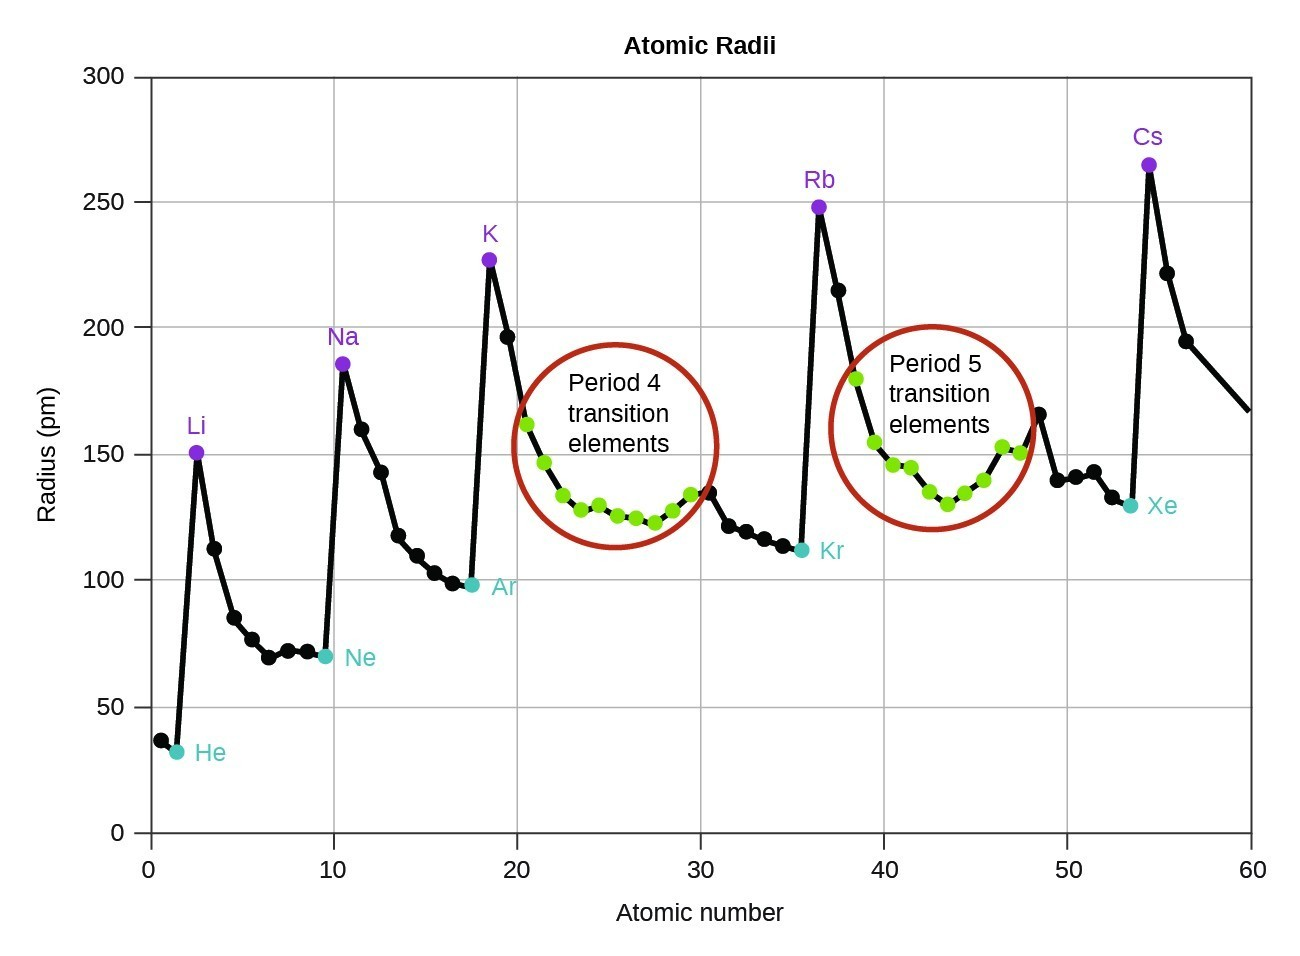
\includegraphics[width=0.45\textwidth,keepaspectratio]{media/atomic_radius_trend.jpg}
\caption{图 原子半径随Z的变化趋势——周期内左到右递减（有效核电荷Zeff增大），族内上到下递增（主量子数n增大）。横轴为原子序数，纵轴为半径(pm)。（普化原理第4版 图11.23）}
\end{figure}

\begin{figure}[H]\centering
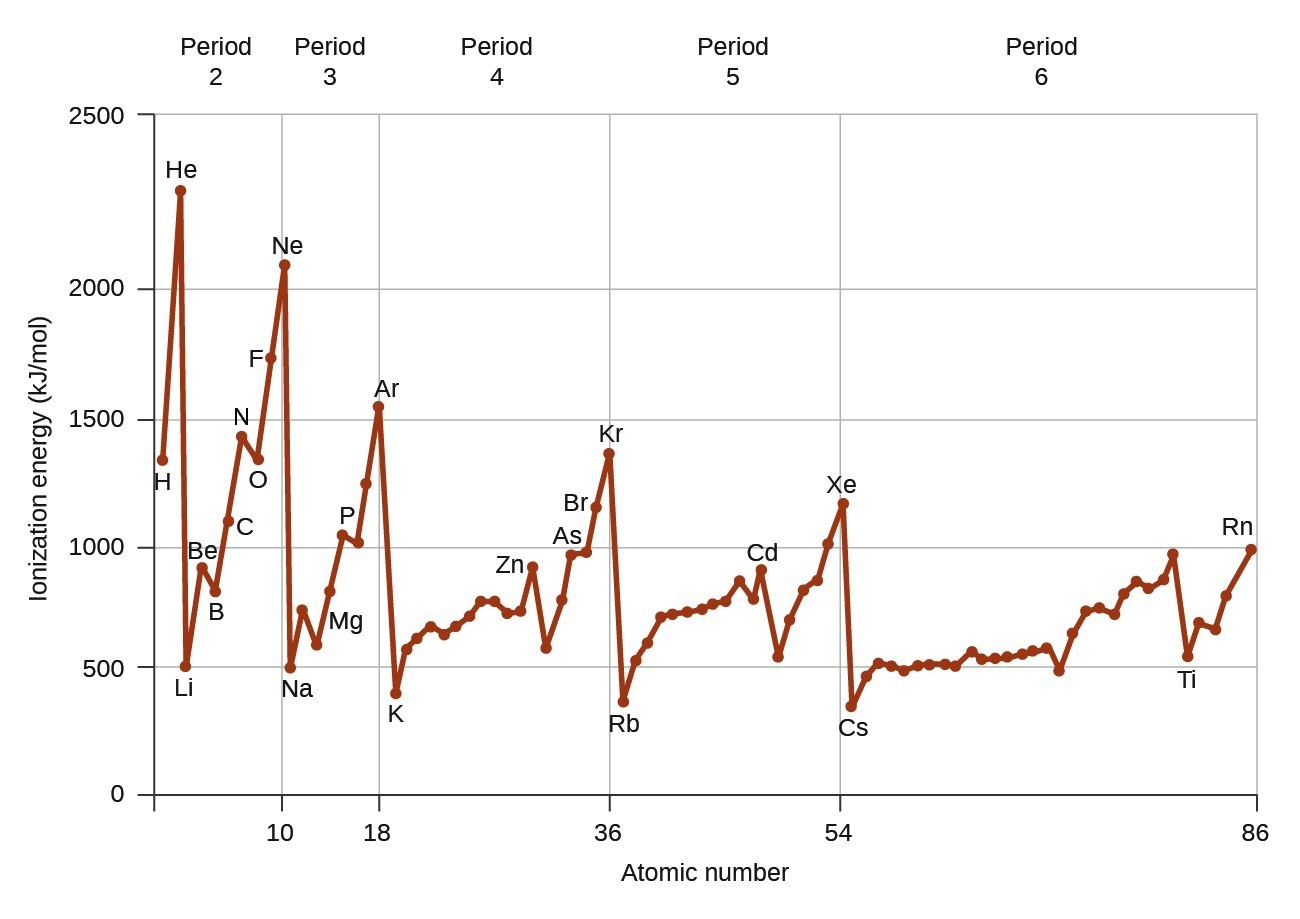
\includegraphics[width=0.45\textwidth,keepaspectratio]{media/first_ionization_energy_trend.jpg}
\caption{图 第一电离能随Z的变化趋势——周期内总体递增（有Be到B和N到O两个凹陷），族内递减。稀有气体始终为周期峰值。横轴为原子序数，纵轴为电离能(kJ/mol)。（普化原理第4版 图11.24）}
\end{figure}

\begin{figure}[H]\centering
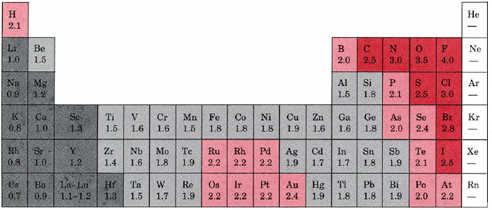
\includegraphics[width=0.45\textwidth,keepaspectratio]{media/electronegativity_table.jpg}
\caption{图 电负性(Pauling标度)随Z的变化趋势——F(4.0)最大，Cs(0.7)最小。周期内左到右递增，族内上到下递减。横轴为原子序数。（普化原理第4版 图11.25）}
\end{figure}

\textbf{四趋势汇总}：

{\def\LTcaptype{none} % do not increment counter
\begin{longtable}[]{@{}lccl@{}}
\toprule\noalign{}
性质 & 周期内（左→右） & 族内（上→下） & 关键机制 \\
\midrule\noalign{}
\endhead
\bottomrule\noalign{}
\endlastfoot
\textbf{原子半径} & ↓ 减小 & ↑ 增大 & \(Z_{eff}\) 增大/ \(n\) 增大 \\
\textbf{第一电离能} & ↑ 增大（有凹陷） & ↓ 减小 & \(Z_{eff}\) 增大/半径增大 \\
\textbf{电负性} & ↑ 增大 & ↓ 减小 & 吸引电子能力 \\
\textbf{电子亲和能} & ↑ 增大（有例外） & ↓ 减小 & 释放能量大小 \\
\end{longtable}
}

\begin{quote}
💡 \textbf{易错提醒}：「比较电离能，先看轨道类型，再看周期趋势」------不看轨道类型直接比周期趋势容易出错，约35\%的同学会在这里翻车。例如 N(\(p^3\) 半满) 的第一电离能 \textgreater{} O(\(p^4\))，这不是周期趋势的反常，而是 Hund 规则的体现。
\end{quote}

\subsubsection{3.7 从原子结构到化学性质：次级周期性}\label{ux4eceux539fux5b50ux7ed3ux6784ux5230ux5316ux5b66ux6027ux8d28ux6b21ux7ea7ux5468ux671fux6027}

学完原子结构，不能只会''比大小''------还要能用它解释元素化学的宏观现象。\textbf{次级周期性}（Secondary Periodicity）就是一个极好的例子。

\textbf{现象}：第四周期和第六周期主族元素的高价化合物，氧化性显著强于同族上下元素。

\textbf{因果链}（从原子结构到具体反应）：

\begin{figure}[H]\centering
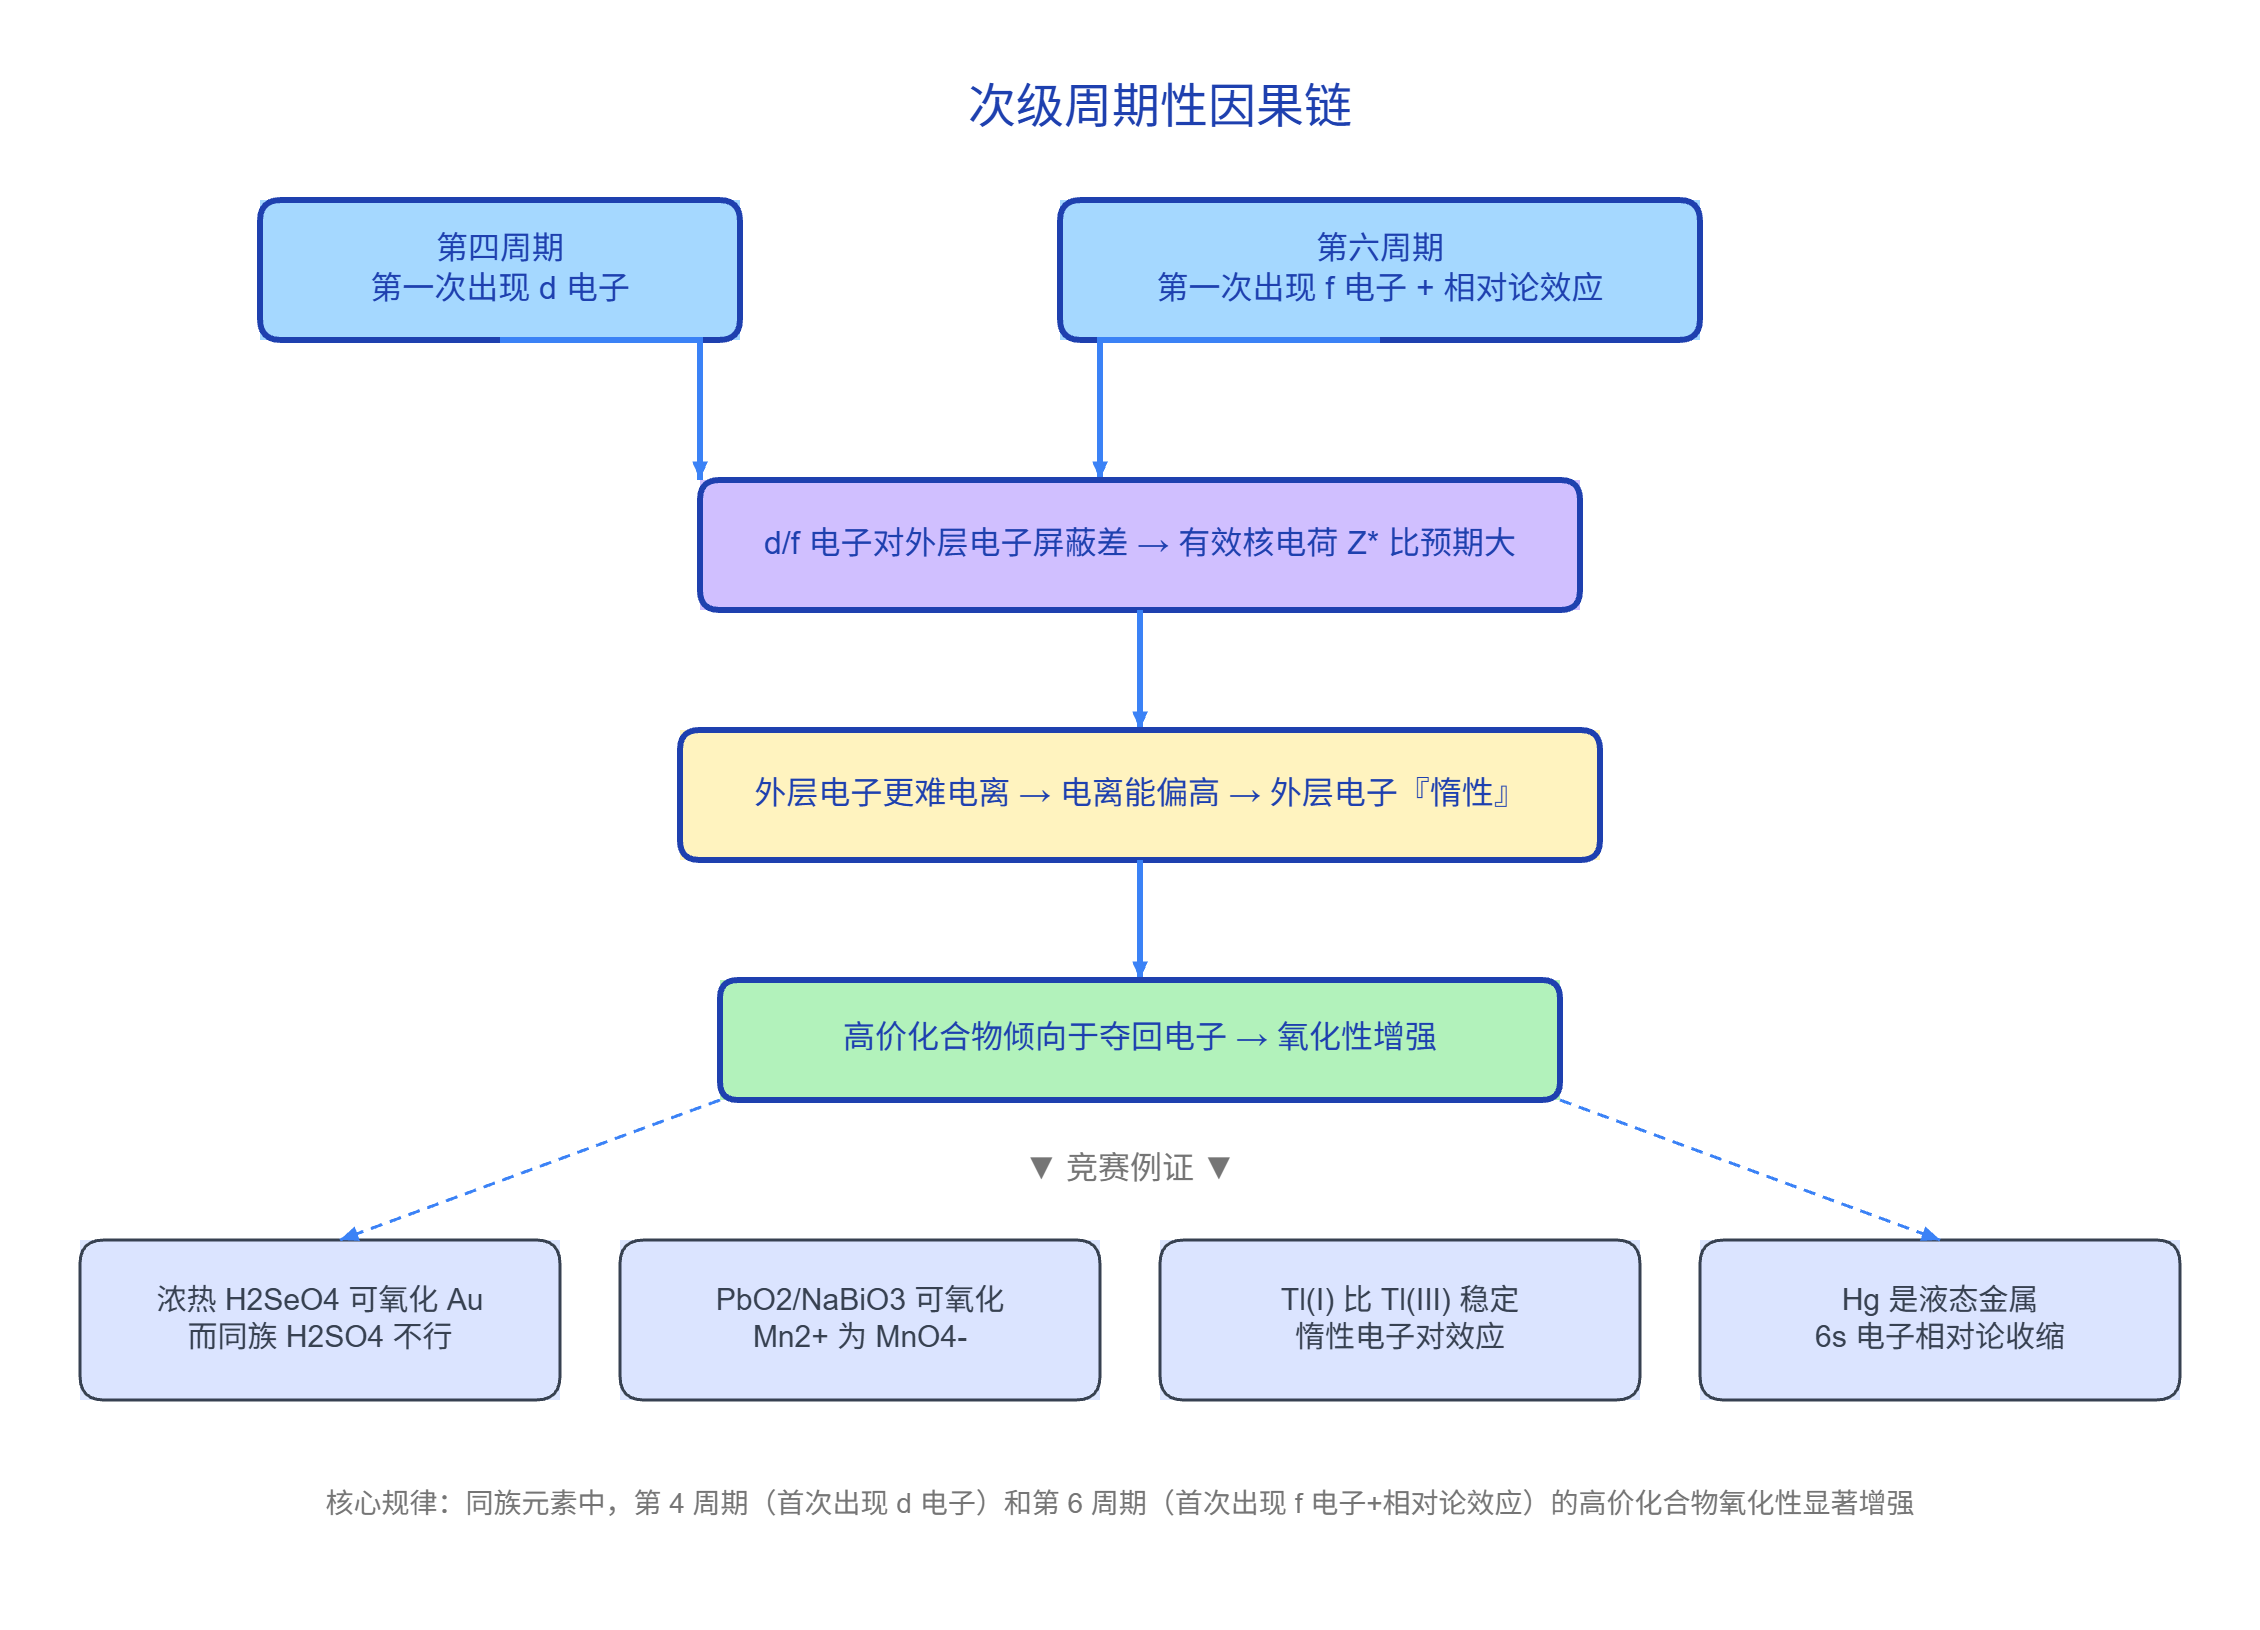
\includegraphics[width=0.5\textwidth,keepaspectratio]{media/次级周期性因果链.causal-chain.png}
\caption{图 次级周期性因果链——从电子构型到氧化性增强的完整逻辑路径：蓝色框为”原因”，黄色框为”中间效应”，绿色框为”化学结果”，底部四个浅蓝框为竞赛级例证}
\end{figure}

\begin{quote}
💡 \textbf{读图提示}：上图中蓝色框为''原因''，黄色框为''中间效应''，绿色框为''化学结果''，底部四个浅蓝框为竞赛级例证。因果链的核心是：\textbf{d/f 电子屏蔽差 → Z* 大 → 电子难电离 → 高价化合物氧化性强}。
\end{quote}

\textbf{竞赛级例证}：
- 浓热 \(H_2SeO_4\) 可氧化 Au（而同族的 \(H_2SO_4\) 不行）
- \(PbO_2\) 和 \(NaBiO_3\) 可把 \(Mn^{2+}\) 氧化为 \(MnO_4^-\)（\(SnO_2\) 和 \(Sb_2O_5\) 无此强氧化性）
- \(Tl(I)\) 比 \(Tl(III)\) 稳定（6s\textsuperscript{2} \textbf{惰性电子对效应}）
- \(Hg\) 的 6s\textsuperscript{2} 不易失去 → \(Hg\) 是液态（6s 电子相对论收缩）

\textbf{这才是''学原子结构有什么用''的答案}：屏蔽/钻穿/有效核电荷这些概念，最终是为了解释元素为什么有那样的化学性质。

\subsection{四、规律与方法}\label{ux56dbux89c4ux5f8bux4e0eux65b9ux6cd5}

\subsubsection{4.1 三类''顺序''的深度辨析}\label{ux4e09ux7c7bux987aux5e8fux7684ux6df1ux5ea6ux8fa8ux6790}

{\def\LTcaptype{none} % do not increment counter
\begin{longtable}[]{@{}
  >{\raggedright\arraybackslash}p{(\linewidth - 6\tabcolsep) * \real{0.2500}}
  >{\raggedright\arraybackslash}p{(\linewidth - 6\tabcolsep) * \real{0.2500}}
  >{\raggedright\arraybackslash}p{(\linewidth - 6\tabcolsep) * \real{0.2500}}
  >{\raggedleft\arraybackslash}p{(\linewidth - 6\tabcolsep) * \real{0.2500}}@{}}
\toprule\noalign{}
\begin{minipage}[b]{\linewidth}\raggedright
顺序类型
\end{minipage} & \begin{minipage}[b]{\linewidth}\raggedright
规则
\end{minipage} & \begin{minipage}[b]{\linewidth}\raggedright
示例（Fe）
\end{minipage} & \begin{minipage}[b]{\linewidth}\raggedleft
口诀
\end{minipage} \\
\midrule\noalign{}
\endhead
\bottomrule\noalign{}
\endlastfoot
\textbf{书写顺序} & 按 \(n\) 由小到大 & {[}Ar{]} 3d\textsuperscript{6}4s\textsuperscript{2} & 写完按n排 \\
\textbf{填充顺序} & 按能量由低到高（Pauling图） & 4s先于3d填 & 先填低能级 \\
\textbf{电离顺序} & 先失 \(n\) 最大的电子 & Fe→Fe\textsuperscript{2+}先失4s\textsuperscript{2} & 失电子找最大n \\
\end{longtable}
}

\subsubsection{4.2 八大常见误区}\label{ux516bux5927ux5e38ux89c1ux8befux533a}

{\def\LTcaptype{none} % do not increment counter
\begin{longtable}[]{@{}cll@{}}
\toprule\noalign{}
\# & 误区 & 正确理解 \\
\midrule\noalign{}
\endhead
\bottomrule\noalign{}
\endlastfoot
1 & ``轨道是电子绕核运动的轨迹'' & \(\|\psi\|^2\) 为概率密度，无确定轨迹 \\
2 & ``\(l\) 取 \(0 \sim n\)'' & \(0 \leq l \leq n-1\) \\
3 & ``离子失电子=填充倒序'' & 先失 \(n\) 最大的电子 \\
4 & ``Cr/Cu特例适用所有类似位置'' & Tc(4d\textsuperscript{5}5s\textsuperscript{2})不遵循Cr模式 \\
5 & ``Pauling图对所有Z成立'' & 填充顺序不变，但Z\textgreater21后 \(E_{3d}<E_{4s}\) \\
6 & ``半充满=绝对最稳定'' & Tc是反例 \\
7 & ``\(m_s=0\) 允许'' & \(m_s\) 必须为 \(\pm1/2\) \\
8 & ``Slater规则精确'' & 对d/f电子误差较大 \\
\end{longtable}
}

\begin{quote}
📝 \textbf{解释题怎么写}
竞赛中有一类''解释题''------不是问''是什么''，而是问''为什么''。这类题的答题质量直接决定区分度：
\textbf{三条铁律}：
1. \textbf{逻辑链条明确}------不要只给结论，要展示因果链：因为 A → 所以 B → 导致 C
2. \textbf{具体分析}------不要说''排斥大''这样的空话，要指出\textbf{谁和谁排斥、为什么排斥、后果是什么}
3. \textbf{简明扼要}------不绕圈子，不写无关信息
\textbf{好答案 vs 坏答案对比}：
\end{quote}

{\def\LTcaptype{none} % do not increment counter
\begin{longtable}[]{@{}
  >{\raggedright\arraybackslash}p{(\linewidth - 4\tabcolsep) * \real{0.3333}}
  >{\raggedright\arraybackslash}p{(\linewidth - 4\tabcolsep) * \real{0.3333}}
  >{\raggedright\arraybackslash}p{(\linewidth - 4\tabcolsep) * \real{0.3333}}@{}}
\toprule\noalign{}
\begin{minipage}[b]{\linewidth}\raggedright
题目
\end{minipage} & \begin{minipage}[b]{\linewidth}\raggedright
❌ 坏答案
\end{minipage} & \begin{minipage}[b]{\linewidth}\raggedright
✅ 好答案
\end{minipage} \\
\midrule\noalign{}
\endhead
\bottomrule\noalign{}
\endlastfoot
碱金属密度为什么不单调？ & ``因为原子半径和质量相互影响'' & ``密度 = 质量/体积。同族向下，质量增加（+14→+16 AMU/周期）的速度快于半径增大（+30\%→+15\%/周期）的增速------因此密度先减后增'' \\
卤素电子亲和能为什么 F\textless Cl？ & ``因为 F 半径小，排斥大'' & ``F 的价层电子云密度极高，加电子后新增电子受到已存在电子的强烈排斥------放出的能量反而低于 Cl'' \\
铁系金属熔点为什么从左到右递减？ & ``因为金属键减弱'' & ``Fe→Co→Ni：3d 轨道中反键电子数增加（6→7→8）→ 金属键中的净成键电子数减少 → 键能下降 → 熔点递减'' \\
\end{longtable}
}

\subsection{五、典型例题}\label{ux4e94ux5178ux578bux4f8bux9898}

\subsubsection{例1 电子排布书写 ⭐⭐}\label{ux4f8b1-ux7535ux5b50ux6392ux5e03ux4e66ux5199}

\textbf{题目}：写出Mg、Cl、Cr、Fe\textsuperscript{2+}的基态电子排布式（稀有气体简式）。

\subsubsection{例2 量子数合法性判断 ⭐⭐⭐}\label{ux4f8b2-ux91cfux5b50ux6570ux5408ux6cd5ux6027ux5224ux65ad}

\textbf{题目}：判断下列量子数组是否可能：(1) n=2,l=2,\(m_l\)=0,m\_s=+1/2；(2) n=3,l=1,\(m_l\)=-1,m\_s=-1/2；(3) n=4,l=0,\(m_l\)=1,m\_s=+1/2；(4) n=3,l=2,\(m_l\)=-2,m\_s=0。

\subsubsection{例3 Balmer系波长计算 ⭐⭐}\label{ux4f8b3-balmerux7cfbux6ce2ux957fux8ba1ux7b97}

\textbf{题目}：计算\(H_\beta\)线（n=4→n=2）波长。\(R_H=1.097\times10^5\ \mathrm{cm^{-1}}\)。

\subsubsection{例4 未成对电子数+磁性 ⭐⭐⭐}\label{ux4f8b4-ux672aux6210ux5bf9ux7535ux5b50ux6570ux78c1ux6027}

\textbf{题目}：计算 N、O、Cl、Mn 原子基态的未成对电子数，并按磁矩从大到小排序。利用公式 \(\mu = \sqrt{n(n+2)}\) 计算各原子的磁矩（B.M.）。

\subsubsection{例5 电离能突变推断族属 ⭐⭐⭐}\label{ux4f8b5-ux7535ux79bbux80fdux7a81ux53d8ux63a8ux65adux65cfux5c5e}

\textbf{题目}：某元素 A 的 I1 到 I5 (kJ/mol)：578, 1817, 2745, 11575, 14830。推断 A 的族属并写出电子排布式。

\subsubsection{例6 过渡金属综合 ⭐⭐⭐⭐}\label{ux4f8b6-ux8fc7ux6e21ux91d1ux5c5eux7efcux5408}

\textbf{题目}：A 为第四周期过渡金属元素，其基态原子有 5 个未成对电子。A\(^{2+}\) 的磁矩小于 A。写出 A 的元素符号、基态排布及 A\(^{2+}\) 中未成对电子数。

\subsubsection{例7 周期律综合推断 ⭐⭐⭐⭐}\label{ux4f8b7-ux5468ux671fux5f8bux7efcux5408ux63a8ux65ad}

\textbf{题目}：三种短周期元素 X、Y、Z。X 的最高价氧化物对应水化物既能与酸又能与碱反应。Y 的阴离子与 Z 的阳离子电子层结构相同。Z 原子序数最大。推断 X、Y、Z。

\begin{center}\rule{0.5\linewidth}{0.5pt}\end{center}

\textbf{例题答案}

\textbf{例1}：Mg={[}Ne{]}3s\textsuperscript{2}；Cl={[}Ne{]}3s\textsuperscript{2}3p\textsuperscript{5}；Cr={[}Ar{]}3d\textsuperscript{5}4s\textsuperscript{1}（半满特例）；Fe\textsuperscript{2+}={[}Ar{]}3d\textsuperscript{6}（先失4s\textsuperscript{2}）

\textbf{例2}：(1) ❌ l\textgreater n-1；(2) ✅ 3p轨道；(3) ❌ \(m_l\)超范围；(4) ❌ m\_s不能为0。

\textbf{例3}：\(\tilde{\nu}=1.097\times10^5\times(1/4-1/16)=20569\ \mathrm{cm^{-1}}\)，\(\lambda=1/20569=486.2\ \mathrm{nm}\)（蓝绿色）。

\textbf{例4}：N 3个，O 2个，Cl 1个，Mn 5个。磁矩：Mn(5.92) \textgreater{} N(3.87) \textgreater{} O(2.83) \textgreater{} Cl(1.73) B.M.

\textbf{例5}：\(I_3\to I_4\)剧增→3个价电子→ⅢA族→Al（\(I_1=578\)与题目580吻合）。

\textbf{例6}：Mn（Z=25），{[}Ar{]}3d\textsuperscript{5}4s\textsuperscript{2}；Mn\textsuperscript{2+} {[}Ar{]}3d\textsuperscript{5}，5未成对，强顺磁性；Mn\textsuperscript{3+} {[}Ar{]}3d\textsuperscript{4}，磁矩减小。

\textbf{例7}：Si、P、Na（第三周期）；Na {[}Ne{]}3s\textsuperscript{1} 氧化态+1；SiCl\textsubscript{4}正四面体。

\subsection{七、本节总结 · 速查}\label{ux4e03ux672cux8282ux603bux7ed3-ux901fux67e5}

{\def\LTcaptype{none} % do not increment counter
\begin{longtable}[]{@{}
  >{\raggedright\arraybackslash}p{(\linewidth - 4\tabcolsep) * \real{0.3333}}
  >{\raggedright\arraybackslash}p{(\linewidth - 4\tabcolsep) * \real{0.3333}}
  >{\raggedright\arraybackslash}p{(\linewidth - 4\tabcolsep) * \real{0.3333}}@{}}
\toprule\noalign{}
\begin{minipage}[b]{\linewidth}\raggedright
核心概念
\end{minipage} & \begin{minipage}[b]{\linewidth}\raggedright
关键规律
\end{minipage} & \begin{minipage}[b]{\linewidth}\raggedright
常见陷阱
\end{minipage} \\
\midrule\noalign{}
\endhead
\bottomrule\noalign{}
\endlastfoot
\textbf{四个量子数} & \(n\): 电子层；\(l\): 形状；\(m_l\): 取向；\(m_s\): 自旋 & \(l\) 最大 n-1 \\
\textbf{电子排布三原则} & Aufbau+Pauli+Hund & 忽略Hund→未成对算错 \\
\textbf{屏蔽效应} & 内层遮挡→\(Z^*\)↓→外层能量↑ & 混淆屏蔽与钻穿 \\
\textbf{钻穿效应} & \(ns>np>nd>nf\) & 钻穿强=能量低 \\
\textbf{能级交错} & \(E_{4s}<E_{3d}\)（填充时） & Z\textgreater21后 \(E_{3d}<E_{4s}\) \\
\textbf{失电子顺序} & 先失 \(n\) 最大电子 & Fe→Fe\textsuperscript{2+}应失4s \\
\textbf{半满/全满} & Cr: 3d\textsuperscript{5}; Cu: 3d\textsuperscript{10} & 非所有适用（Tc反例） \\
\end{longtable}
}

\subsection{八、练习题}\label{ux516bux7ec3ux4e60ux9898}

\subsubsection{8.1 基础巩固}\label{ux57faux7840ux5de9ux56fa}

\begin{enumerate}
\def\labelenumi{\arabic{enumi}.}
\tightlist
\item
  写出Na、Mg、Al、Si、P、S、Cl、Ar、K、Ca、Fe、Zn的基态电子排布式。
\item
  计算C、N、O、F、Cl、Fe\textsuperscript{3+}的未成对电子数。
\item
  判断量子数是否可能（略）。
\item
  用Slater规则计算Na的1s、2p、3s电子的 \(Z^*\) 和 \(E\)。
\end{enumerate}

\subsubsection{8.2 提高训练}\label{ux63d0ux9ad8ux8badux7ec3}

\begin{enumerate}
\def\labelenumi{\arabic{enumi}.}
\setcounter{enumi}{4}
\tightlist
\item
  Cr和Cu的排布解释及Mo/Ag迁移。
\item
  Fe→Fe\textsuperscript{2+}→Fe\textsuperscript{3+}和Cu→Cu\textsuperscript{+}→Cu\textsuperscript{2+}的排布变化。
\item
  轨道容量计算（n=5, 5g亚层, 第8周期元素数）。
\item
  计算Paschen系n\textsubscript{2}=5谱线波长。
\end{enumerate}

\subsubsection{8.3 挑战题}\label{ux6311ux6218ux9898}

\begin{enumerate}
\def\labelenumi{\arabic{enumi}.}
\setcounter{enumi}{8}
\tightlist
\item
  电离能推断（\(I_1\)-\(I_5\)数据）。
\item
  {[}Xe{]}4f\textsuperscript{14}5d\textsuperscript{10}6s\textsuperscript{1}综合推断。
\item
  Slater规则比较Fe中3d和4s的Z*，解释失电子顺序。
\item
  {[}Koopmans能量分解·Sc排布{]} Sc（Z=21）有三种可能的价电子排布：(a) 3d\textsuperscript{1}4s\textsuperscript{2}, (b) 3d\textsuperscript{2}4s\textsuperscript{1}, (c) 3d\textsuperscript{3}4s\textsuperscript{0}。已知以下实验电离能数据（以Ar为能量零点）：

  \begin{itemize}
  \tightlist
  \item
    Sc\textsuperscript{2+}(3d\textsuperscript{1}) → Sc\textsuperscript{3+} + e\textsuperscript{-}，I = 24.75 eV
  \item
    Sc\textsuperscript{2+}(4s\textsuperscript{1}) → Sc\textsuperscript{3+} + e\textsuperscript{-}，I = 21.60 eV
  \item
    Sc\textsuperscript{+}(3d\textsuperscript{1}4s\textsuperscript{1}) → Sc + e\textsuperscript{-}，E = -6.62 eV（注意：此处为总能量，直接代入方程组）
  \item
    Sc\textsuperscript{+}(4s\textsuperscript{2}) → Sc + e\textsuperscript{-}，E = -7.98 eV
  \item
    Sc(3d\textsuperscript{2}4s\textsuperscript{1}) 与 Sc(3d\textsuperscript{1}4s\textsuperscript{2}) 的能量差 ΔE = 2.03 eV
    设轨道能 U\textsubscript{3}（3d）、U\textsubscript{4}（4s）；电子排斥参数 \(J_{dd}\)（d-d）、\(J_{ds}\)（d-s）、\(J_{ss}\)（s-s）。利用 Koopmans 定理（I ≈ -U）列出方程，解出五个参数，判断哪种排布能量最低。
  \end{itemize}
\end{enumerate}

\subsection{九、参考答案与提示}\label{ux4e5dux53c2ux8003ux7b54ux6848ux4e0eux63d0ux793a}

\textbf{8.1}

\begin{enumerate}
\def\labelenumi{\arabic{enumi}.}
\item
  参见§3.3排布表。
\item
  C:2, N:3, O:2, F:1, Cl:1, Fe\textsuperscript{3+}:5。
\item
  (1)❌ l\textgreater n-1 (2)✅ (3)❌ \(m_l\)超范围。
\item
  Na: 1s σ=0.30 Z\emph{=10.70 E=-1557eV; 2s/2p σ=4.15 Z}=6.85 E=-160eV; 3s σ=8.80 Z*=2.20 E=-7.3eV。
\end{enumerate}

\textbf{8.2}

\begin{enumerate}
\def\labelenumi{\arabic{enumi}.}
\setcounter{enumi}{4}
\item
  Cr:{[}Ar{]}3d\textsuperscript{5}4s\textsuperscript{1}; Cu:{[}Ar{]}3d\textsuperscript{10}4s\textsuperscript{1}; Mo:4d\textsuperscript{5}5s\textsuperscript{1}; Ag:4d\textsuperscript{10}5s\textsuperscript{1}。
\item
  Fe{[}Ar{]}3d\textsuperscript{6}4s\textsuperscript{2}→Fe\textsuperscript{2+}{[}Ar{]}3d\textsuperscript{6}(失4s\textsuperscript{2})→Fe\textsuperscript{3+}{[}Ar{]}3d\textsuperscript{5}; Cu{[}Ar{]}3d\textsuperscript{10}4s\textsuperscript{1}→Cu\textsuperscript{+}{[}Ar{]}3d\textsuperscript{10}→Cu\textsuperscript{2+}{[}Ar{]}3d\textsuperscript{9}。
\item
  (1)50 (2)9轨道18电子 (3)50种。
\item
  7804cm\textsuperscript{-1}, 1281nm(红外)。
\end{enumerate}

\textbf{8.3}

\begin{enumerate}
\def\labelenumi{\arabic{enumi}.}
\setcounter{enumi}{8}
\item
  4个价电子→ⅣA→第三周期Si。
\item
  Z=79 Au; 第六周期ⅠB ds区; +1/+3; Au\textsuperscript{+}反磁性。
\item
  4s Z\emph{=8.85\textgreater3d Z}=6.25, 但E\textsubscript{4}s∝8.85\textsuperscript{2}/16=4.90, E\textsubscript{3}d∝6.25\textsuperscript{2}/9=4.34, 故E\textsubscript{4}s\textgreater E\textsubscript{3}d→先失4s。
\item
  设U\textsubscript{3}(3d轨道能)、U\textsubscript{4}(4s轨道能)、\(J_{dd}\)(d-d排斥)、\(J_{ds}\)(d-s排斥)、\(J_{ss}\)(s-s排斥)。方程组：(1) U\textsubscript{3}=-24.75; (2) U\textsubscript{4}=-21.60; (3) U\textsubscript{4}+\(J_{ds}\)+\(J_{ss}\)=-6.62; (4) U\textsubscript{3}+2\(J_{ds}\)=-7.98; (5) U\textsubscript{3}-U\textsubscript{4}+\(J_{dd}\)-\(J_{ss}\)=2.03。解得U\textsubscript{3}=-24.75, U\textsubscript{4}=-21.60, \(J_{ds}\)=8.39, \(J_{ss}\)=6.60, \(J_{dd}\)=11.78。E(3d\textsuperscript{1}4s\textsuperscript{2})=U\textsubscript{3}+2U\textsubscript{4}+2\(J_{ds}\)+\(J_{ss}\)=-44.59; E(3d\textsuperscript{2}4s\textsuperscript{1})=2U\textsubscript{3}+U\textsubscript{4}+\(J_{dd}\)+2\(J_{ds}\)=-42.56; E(3d\textsuperscript{3}4s\textsuperscript{0})=3U\textsubscript{3}+3\(J_{dd}\)=-38.91。\textbf{结论}：3d\textsuperscript{1}4s\textsuperscript{2}能量最低→虽是3d单电子能(-24.75)低于4s(-21.60)，但d-d排斥(11.78)远大于s-s排斥(6.60)，体系优先填排斥小的4s轨道。
\end{enumerate}

\subsection{十、延伸阅读}\label{ux5341ux5ef6ux4f38ux9605ux8bfb}

\begin{itemize}
\tightlist
\item
  宋天佑《无机化学》§5、张丽荣《无机化学》§5
\item
  上海中学竞赛课程·化学·第一分册·第二讲
\item
  普化原理第4版 Ch11------核化学与放射性（Ch11核反应部分）、电子云的径向分布与角度分布（Ch11 §11.3-11.4）、Cotton Chemical Applications of Group Theory
\end{itemize}
